\documentclass[11pt]{article}

\usepackage{classDM17}
\usepackage{mathtools}
\DeclarePairedDelimiter\ceil{\lceil}{\rceil}
\DeclarePairedDelimiter\floor{\lfloor}{\rfloor}

\title{Asmt 3: Clustering}
\author{Gopal Menon\\Turn in through Canvas by 2:45pm: \\
Wednesday, March 01}
\date{}

\begin{document}
\maketitle



\section{Hierarchical Clustering (20 points)}

\paragraph{A: (20 points)} 

Single-link clustering will tend to form clusters that are larger. The reason is that when the distance between clusters is the closest distance between parts of two clusters, even if other cluster components are spread out, the closest components will determine whether to merge or not. This can be seen in figure \ref{SLC} with the pink cluster ( The four clusters are shown in four different colors.). The opposite effect can be seen in figure \ref{CLC} where the clusters are smaller in the case of the complete-link measure that measures the longest link. The three variants all seem to have done a good job. The points on the top left were separated out by all three methods as part of a cluster. The bottom left and top right points have also been separated out.\\

Both the single-link and complete-link distances will be the easiest to compute through use of a priority queue that stores the distance between pairs of clusters since the queue can be sorted on the shortest or the longest distance. The mean-link computation takes the most time since it has to find the distance between all points in two clusters.

\begin{figure}[!htb]
\centering
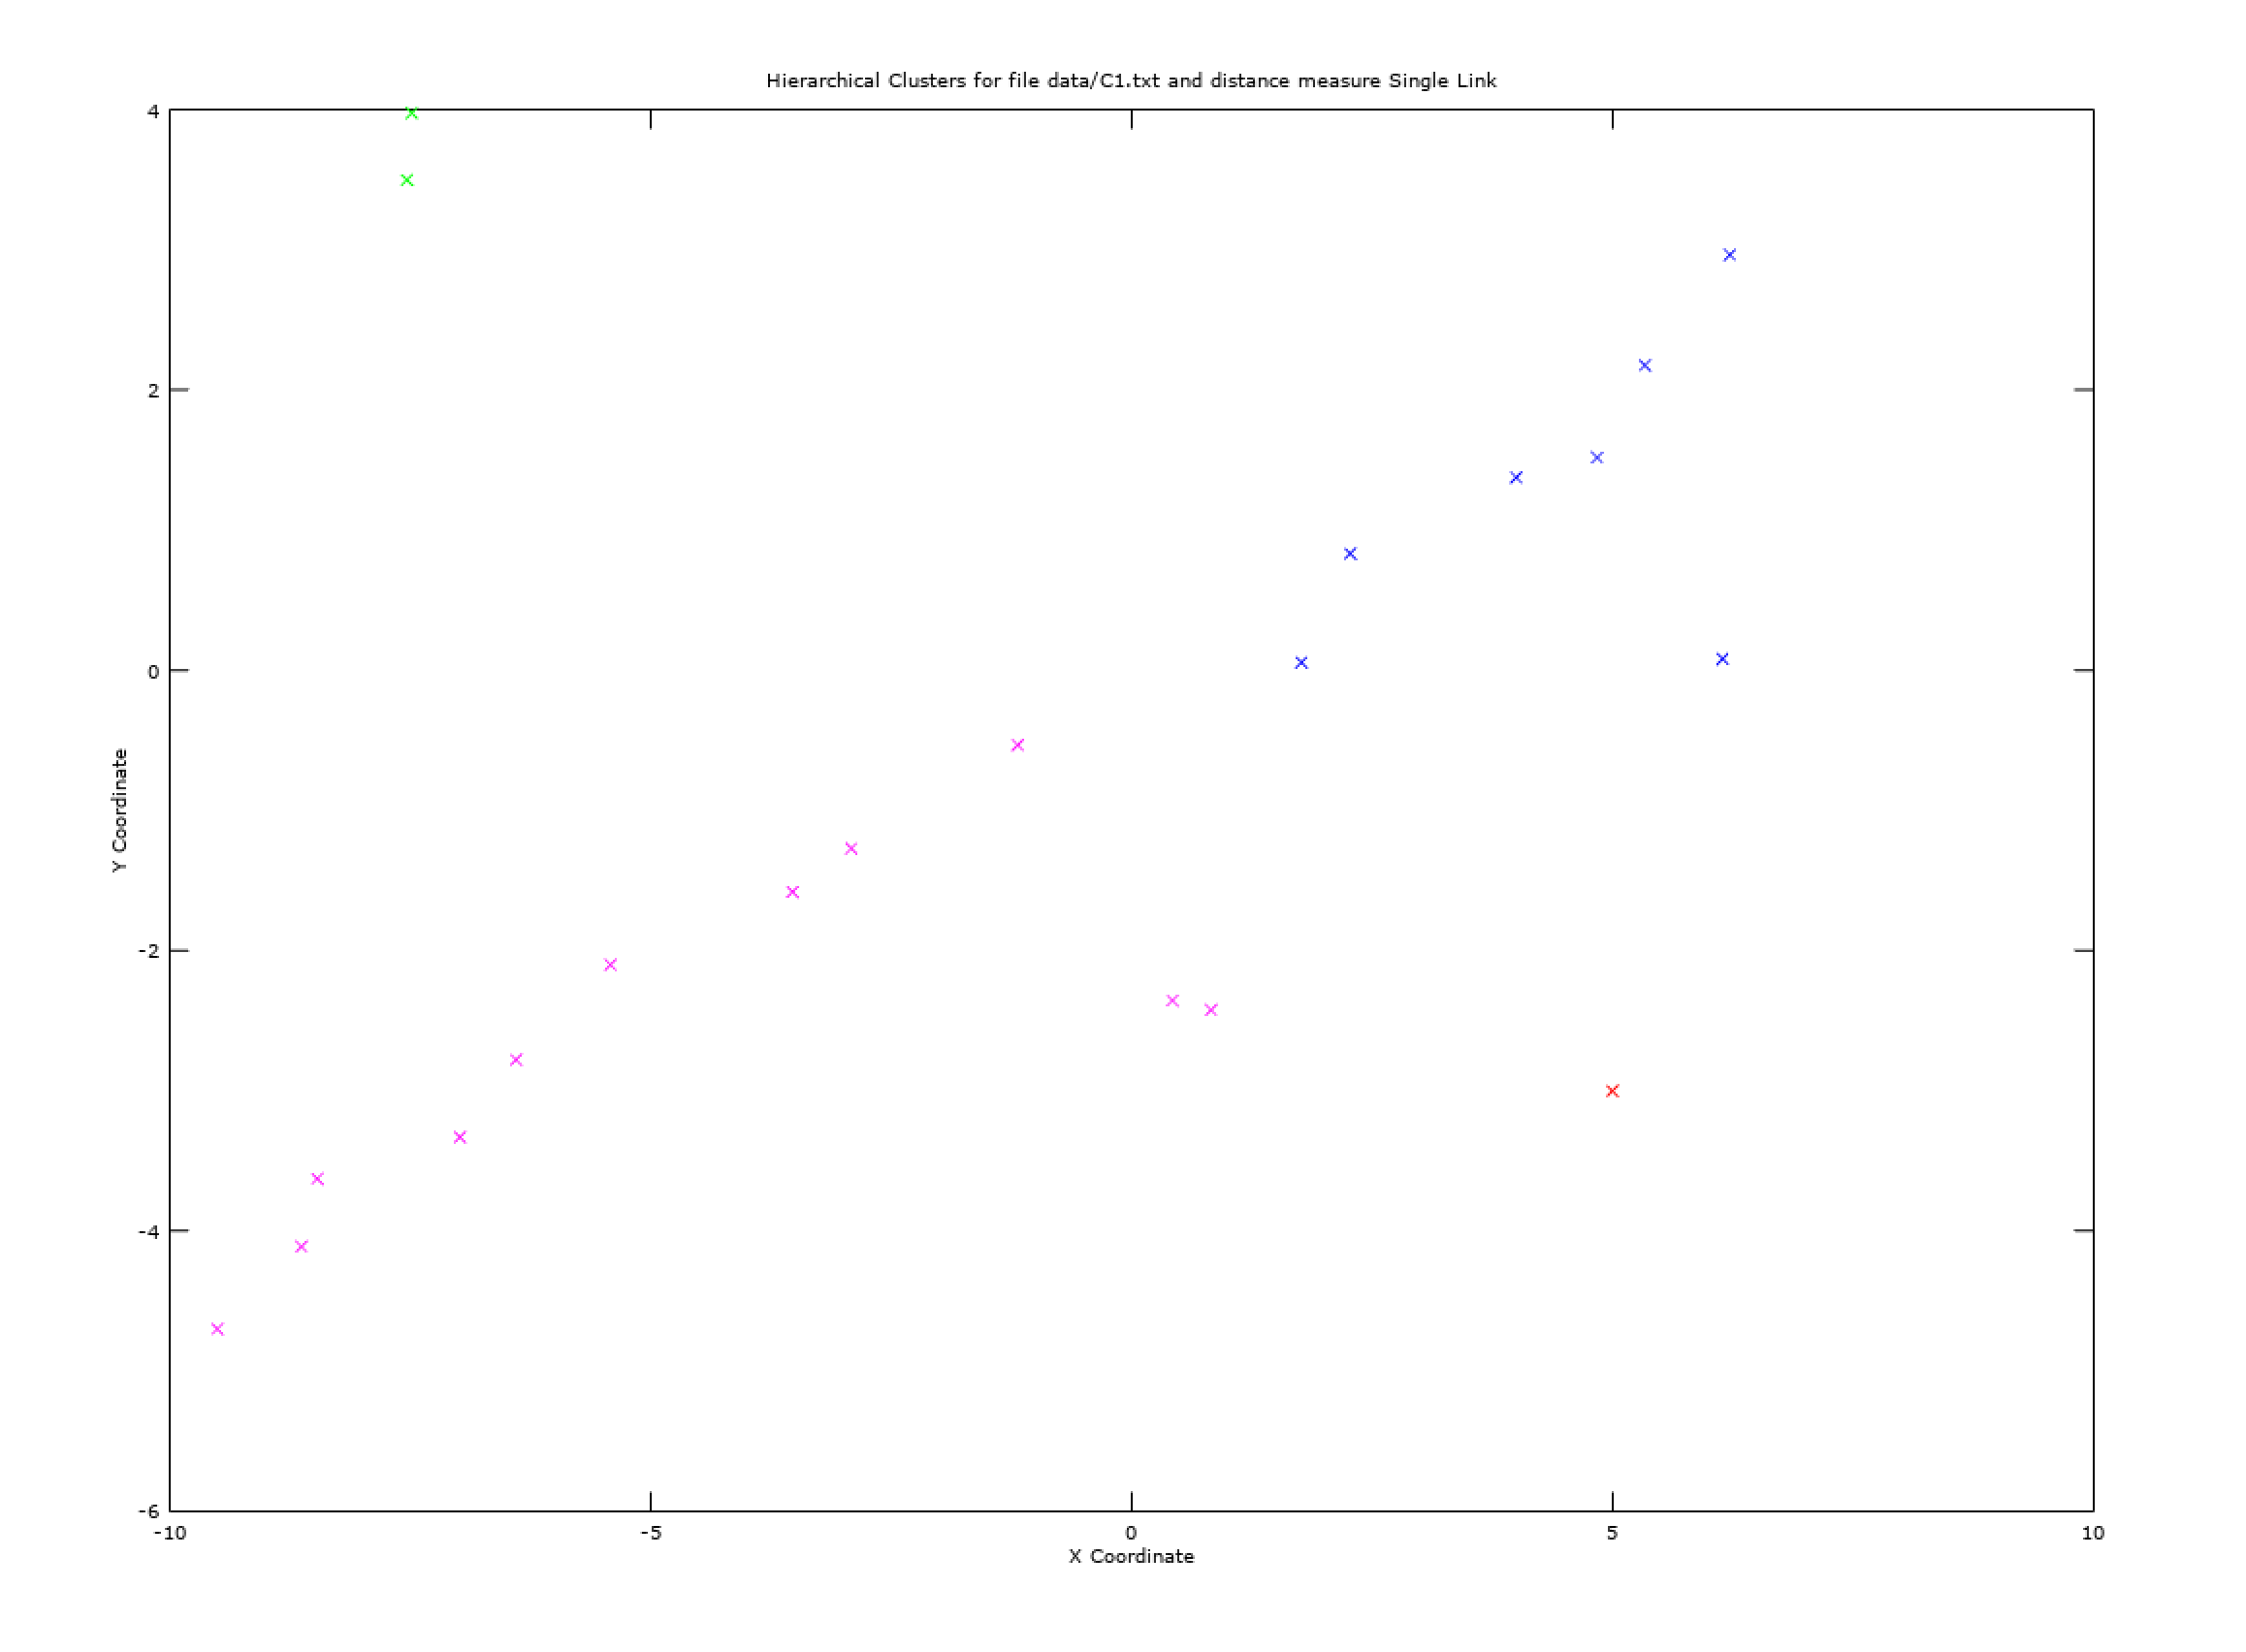
\includegraphics[width=5in]{figures/1ASingleLink.png}
\caption{Single Link Distance Measure Clustering}
\label{SLC}
\end{figure}
 
\begin{figure}[!htb]
\centering
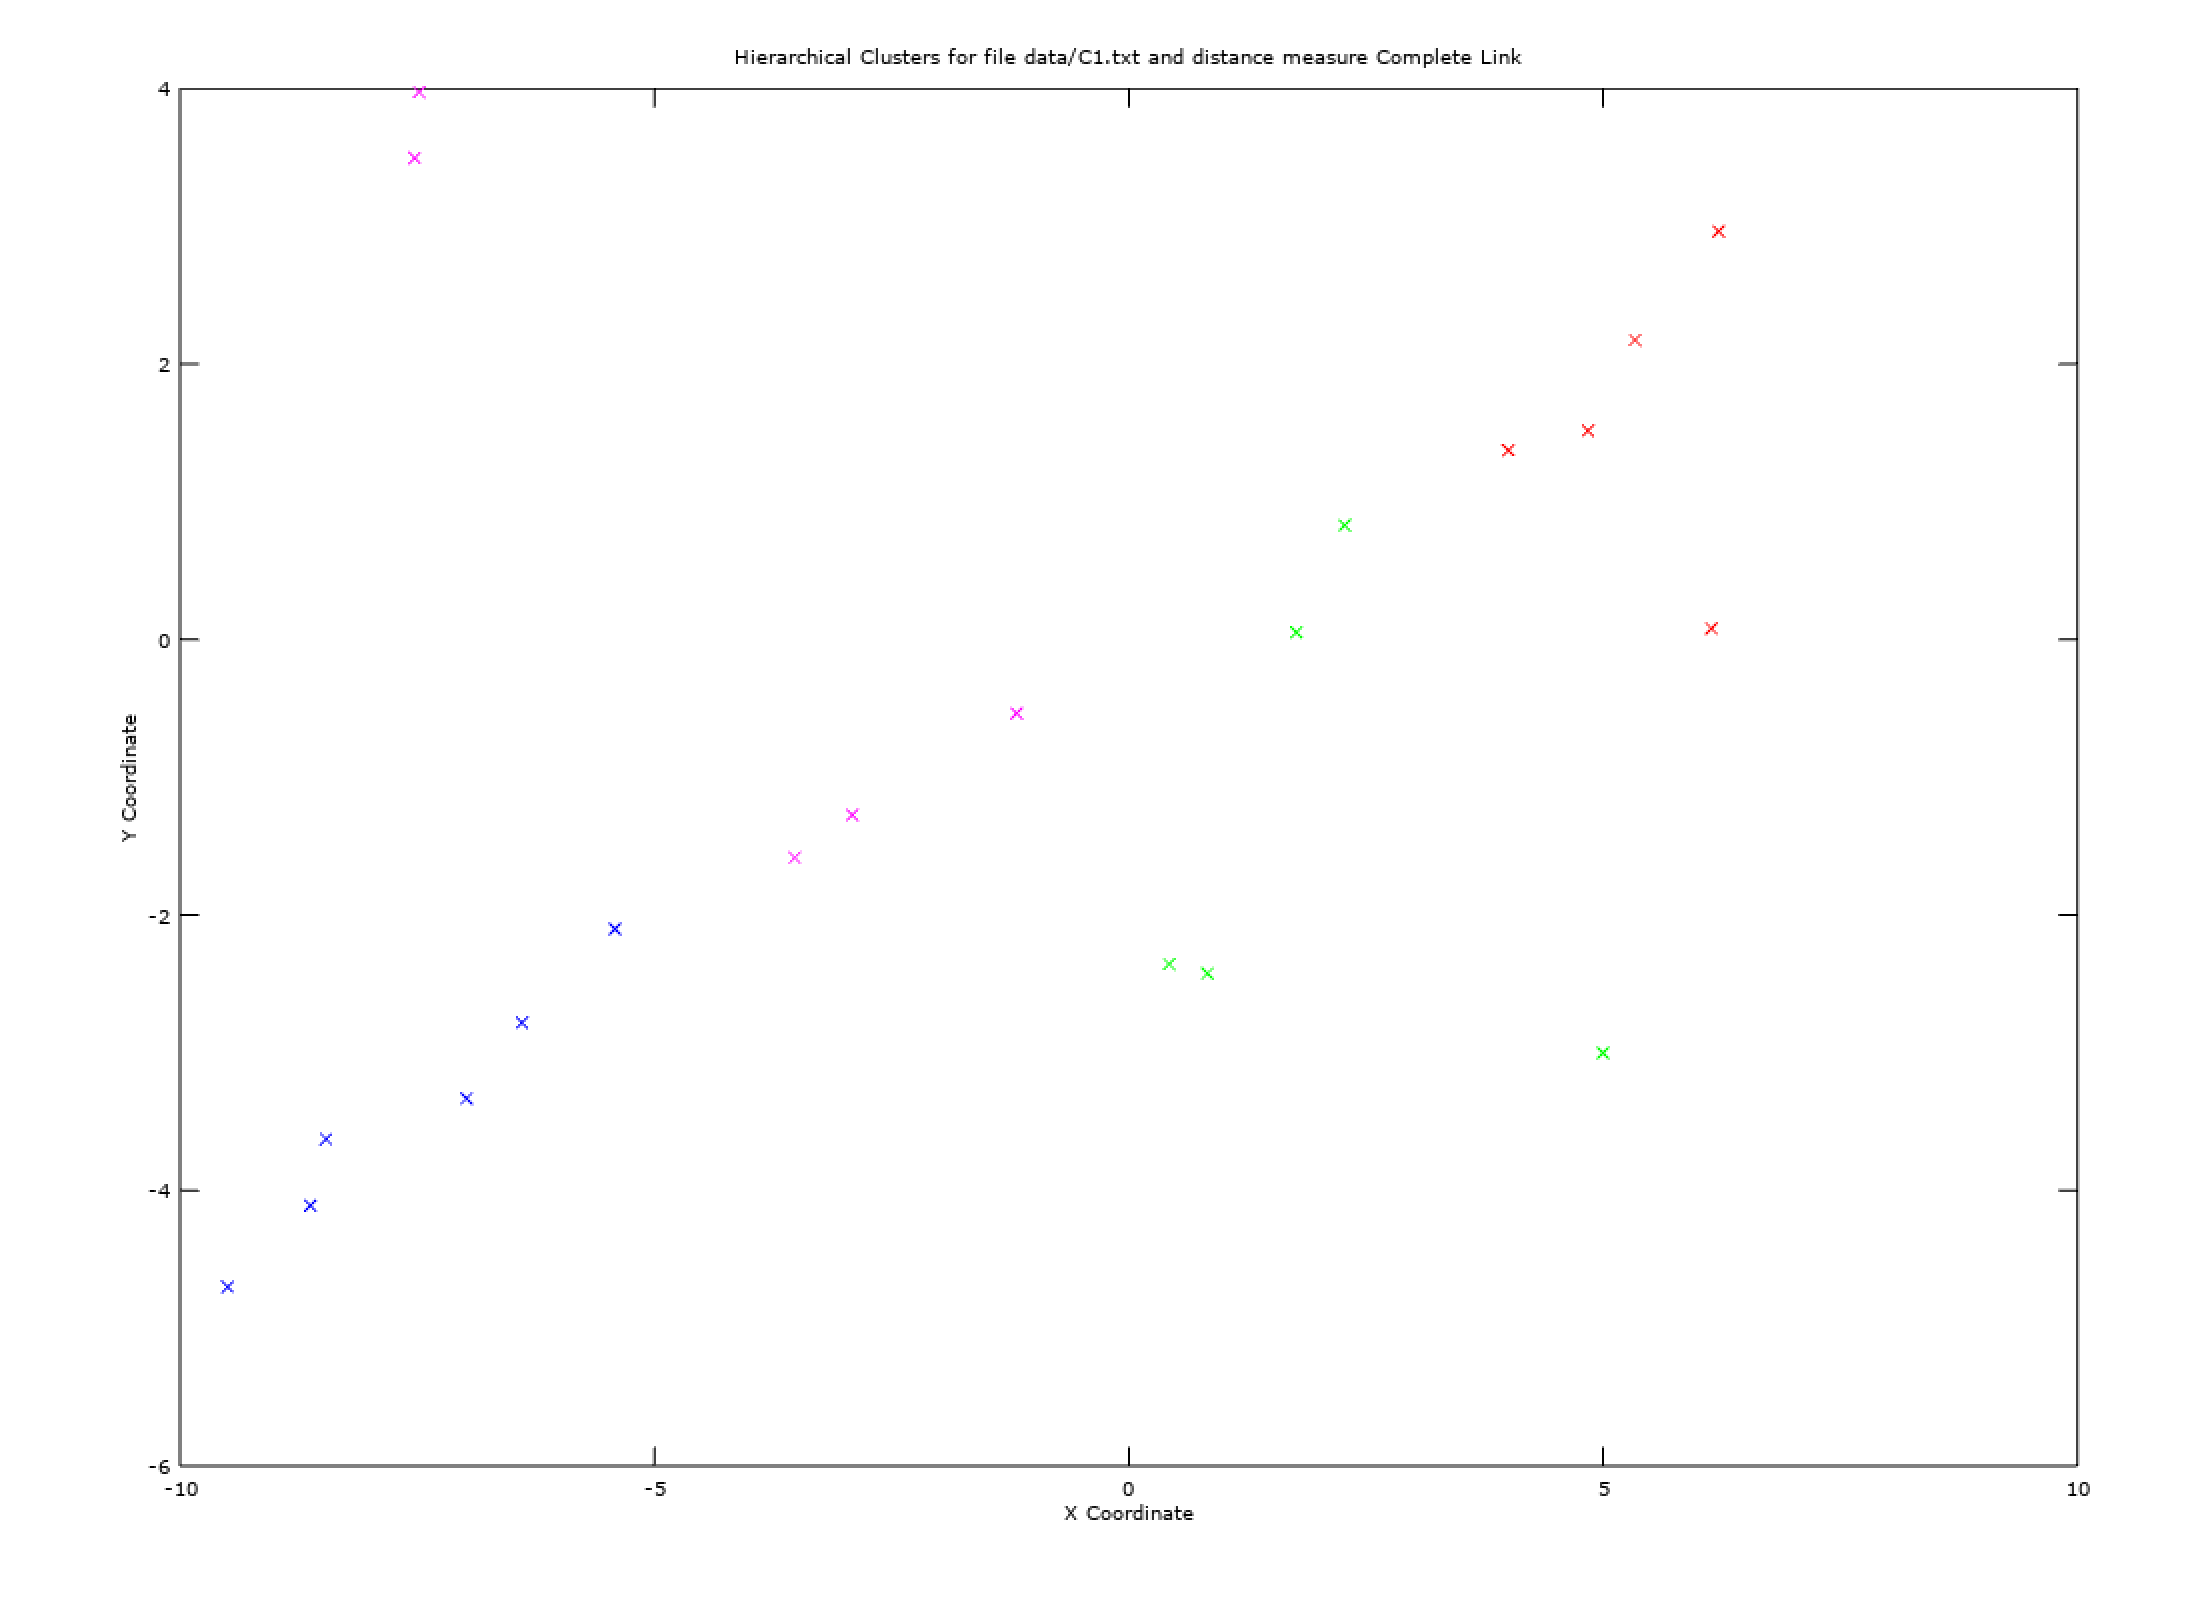
\includegraphics[width=5in]{figures/1ACompleteLink.png}
\caption{Complete Link Distance Measure Clustering}
\label{CLC}
\end{figure}

\begin{figure}[!htb]
\centering
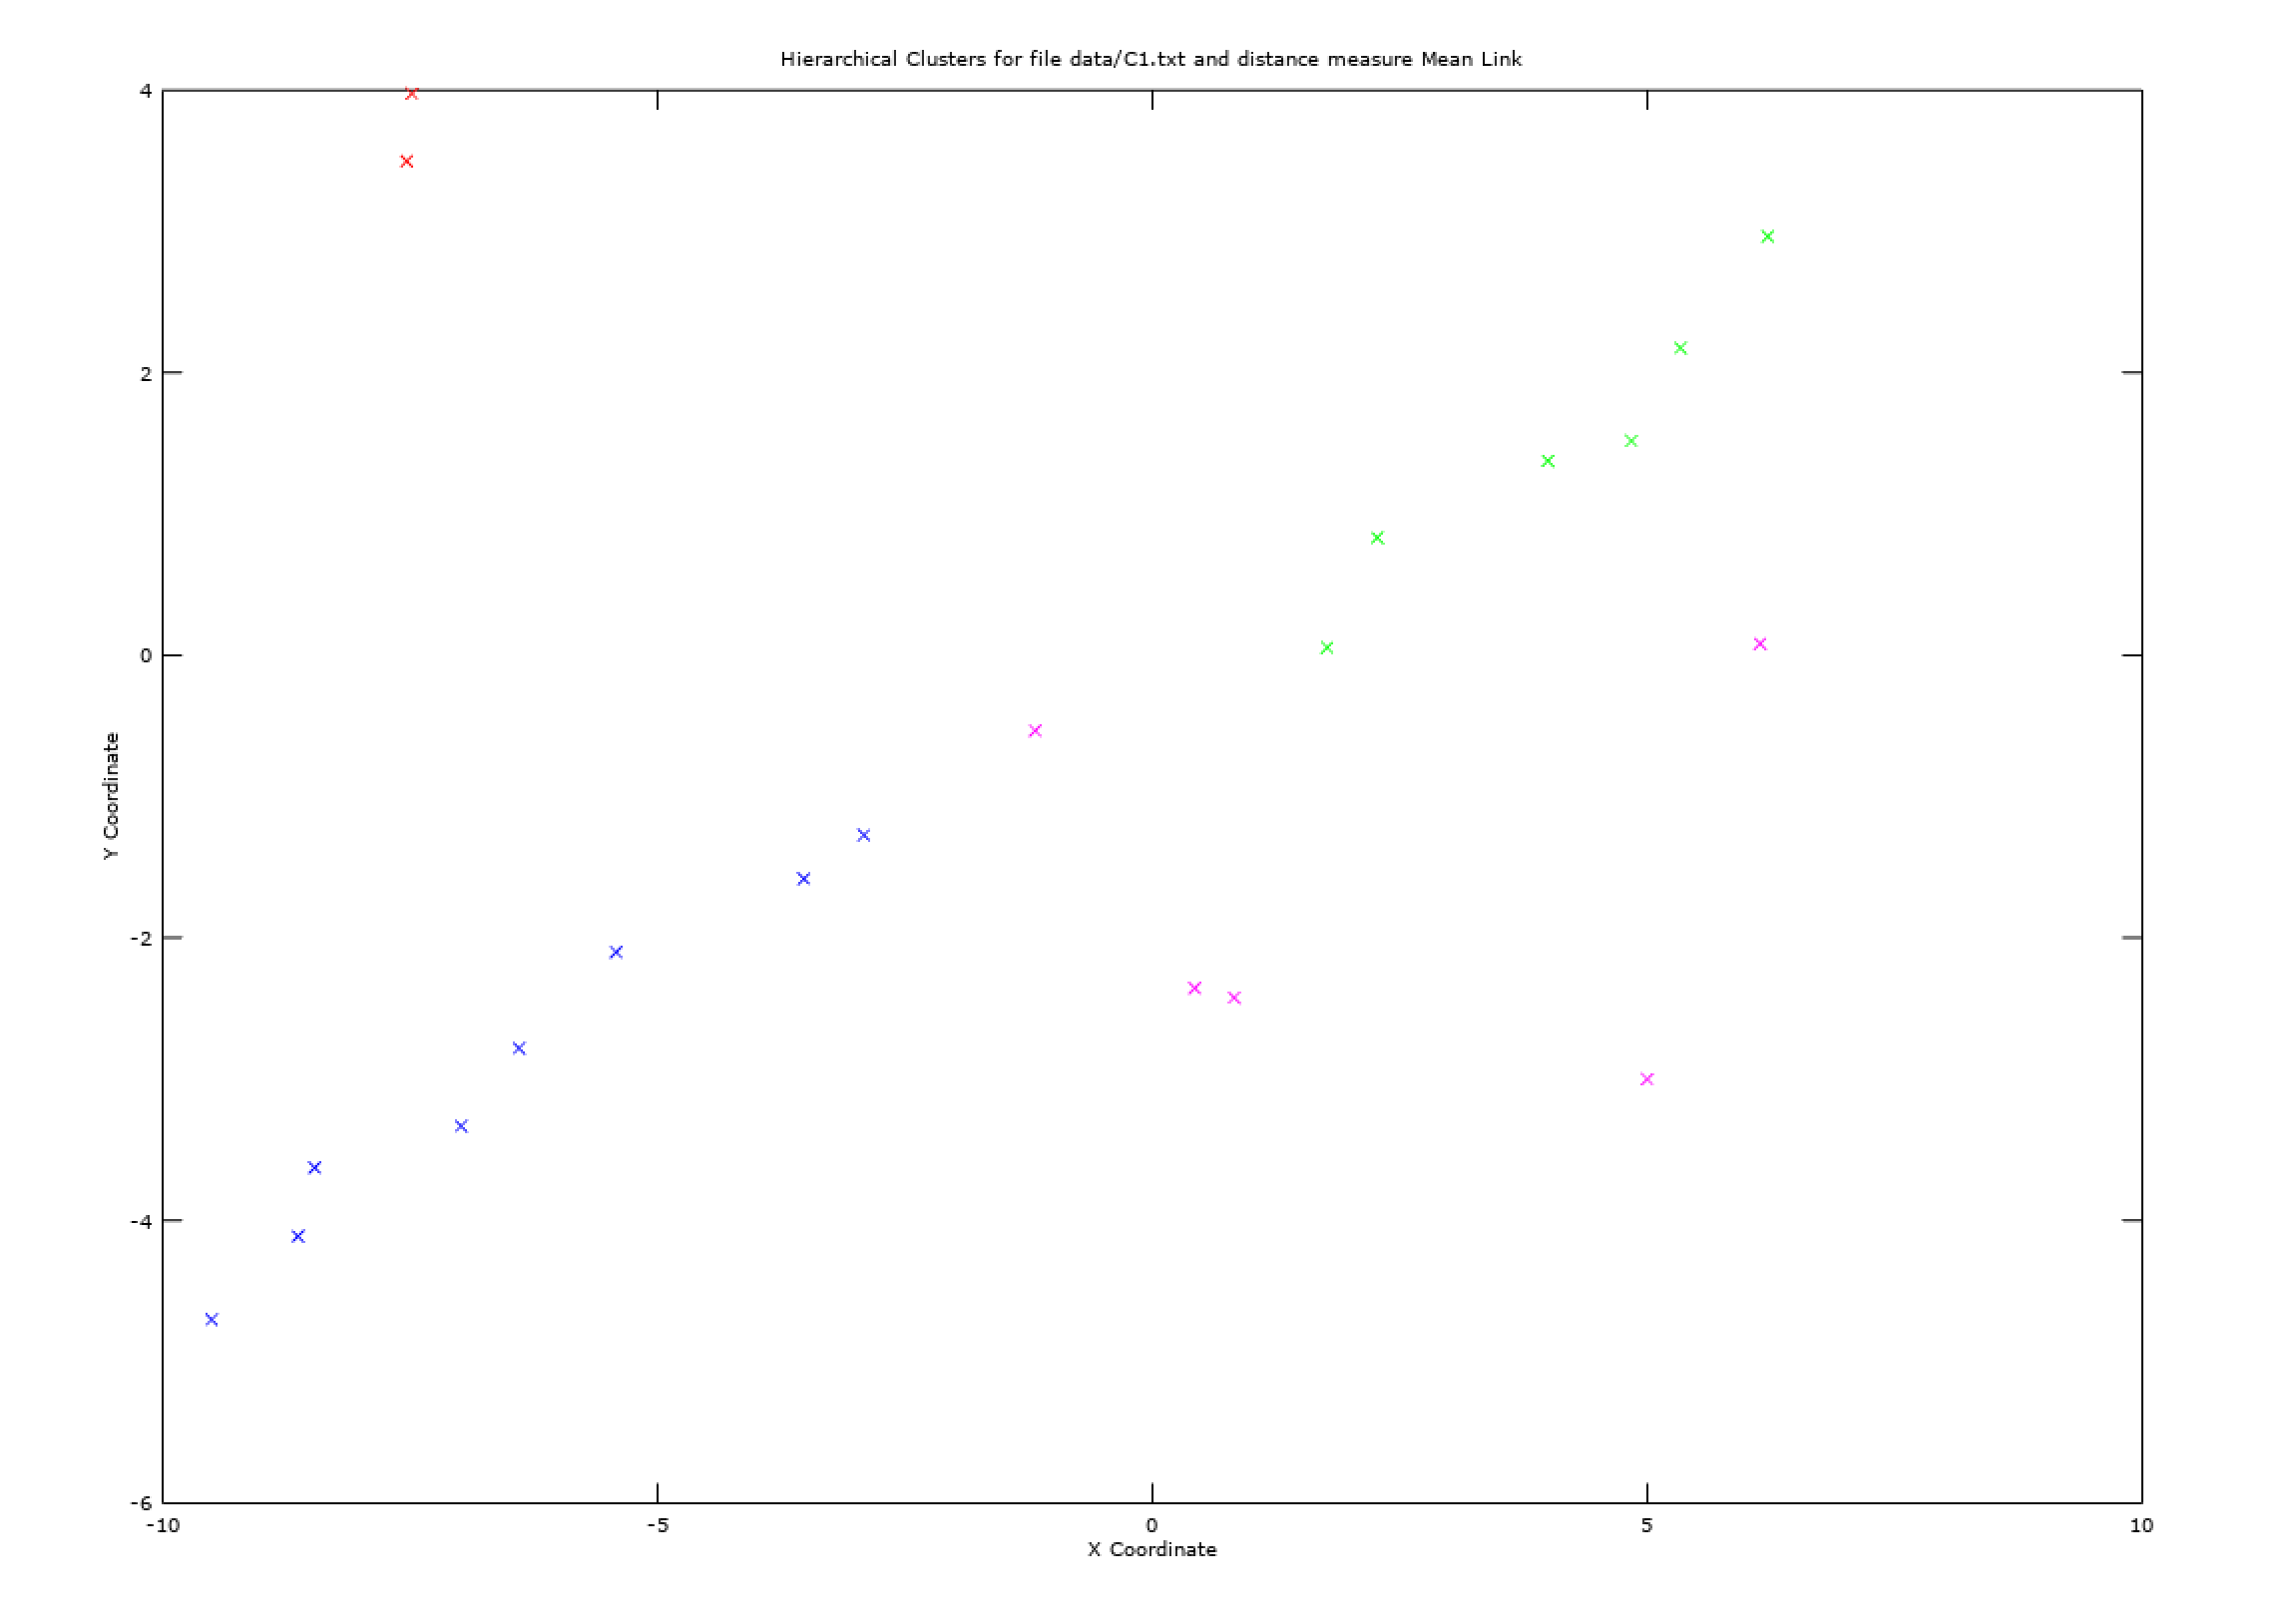
\includegraphics[width=5in]{figures/1AMeanLink.png}
\caption{Mean Link Distance Measure Clustering}
\label{MLC}
\end{figure}

\section{Assignment-Based Clustering (40 points)}

\paragraph{A: (20 points)} 

    \begin{table}[!h] 
    \centering
    \caption{Coordinates for cluster centers}
    \label{table:coords1}
    \begin{tabular}{|c|c|c|c|c|c|}
      \hline
   Algorithm  & Red  Cluster&  Green Cluster & Blue Cluster & 3-Center Cost & 3-Means Cost \\
      \hline      
      Gonzalez &   $(11.7967, 49.4673)$              &  $(110.9812, 88.8712)$  &          $(67.9411, 19.6297)$      & $61.8281$ & $27.8837$                     \\
      \hline      
      K-Means++ &    $(11.7967, 49.4673)$             & $(63.0189, 16.5108)$   &           $(62.0994, 81.2857)$  & $49.4669$ & $8.8481$                       \\
      \hline      
    \end{tabular}
    \end{table}
    
The result of clustering using the Gonzalez algorithm is shown in figure \ref{Gonzalez}. The cluster centers are identified by circles and the components of the clusters are marked by x's. The three clusters are shown in three different colors. The center for the red cluster is not visible since it is obscured by the cluster components crowded together. The result has been affected by the center of the green cluster, which seems to be an outlier. The groups of points in the top middle are shown as part of two clusters. The reason it was not identified as one cluster is because the first point in the file was chosen as a center. The boundary of the Voronoi cell between the red and green clusters is clearly visible in the group of points in the top middle.\\

The result from one iteration of the K-Means++ algorithm is shown in figure \ref{KMPP}. The centers of the red and green clusters are obscured by other points in the cluster, but the center of the blue cluster can be seen if you look carefully. This time since the outlier point was not chosen as a center (since the center is chosen with probability proportional to the distance from the existing centers), the clusters look more accurate when compared to output produced by the Gonzalez algorithm.\\

The coordinate for the centers of the clusters are given in table \ref{table:coords1}. The same table also has the 3-Center and 3-Means costs. The former is the maximum distance between the cluster center and any cluster component. The outlier point seems to be the reason for the high cost. Its higher in the Gonzalez case where all the points are far from the green cluster center. The same cluster in the case of K-Means++ (this time in blue color), is responsible for the high number, again due to the outlier point. The 3-Means cost is the square root of the normalized sum of the squares of the distances between the cluster center and components. Its lower in the case of K-Means++ as the center is within the group of blue points and is not the outlier point.\\

Figure \ref{KPPCum} shows the 3-Means cost and cumulative cost trends over $25$ iterations of the K-Means++ algorithm.\\

Figure \ref{2BOverlap} shows cluster overlap percentage between Gonzalez and K-Means++ clustering. Lines for Clusters 1 and 2 lie on top of one another and so appear as one line. The 100\% overlap of clusters between the two algorithms is for the clusters on the middle left and bottom middle (disregard the cluster color in the legend for figure \ref{2BOverlap}). The low overlap percentage is for the common components of the green cluster in Gonzalez clustering and the blue cluster in K-Means++ clustering.

\begin{figure}[!htb]
\centering
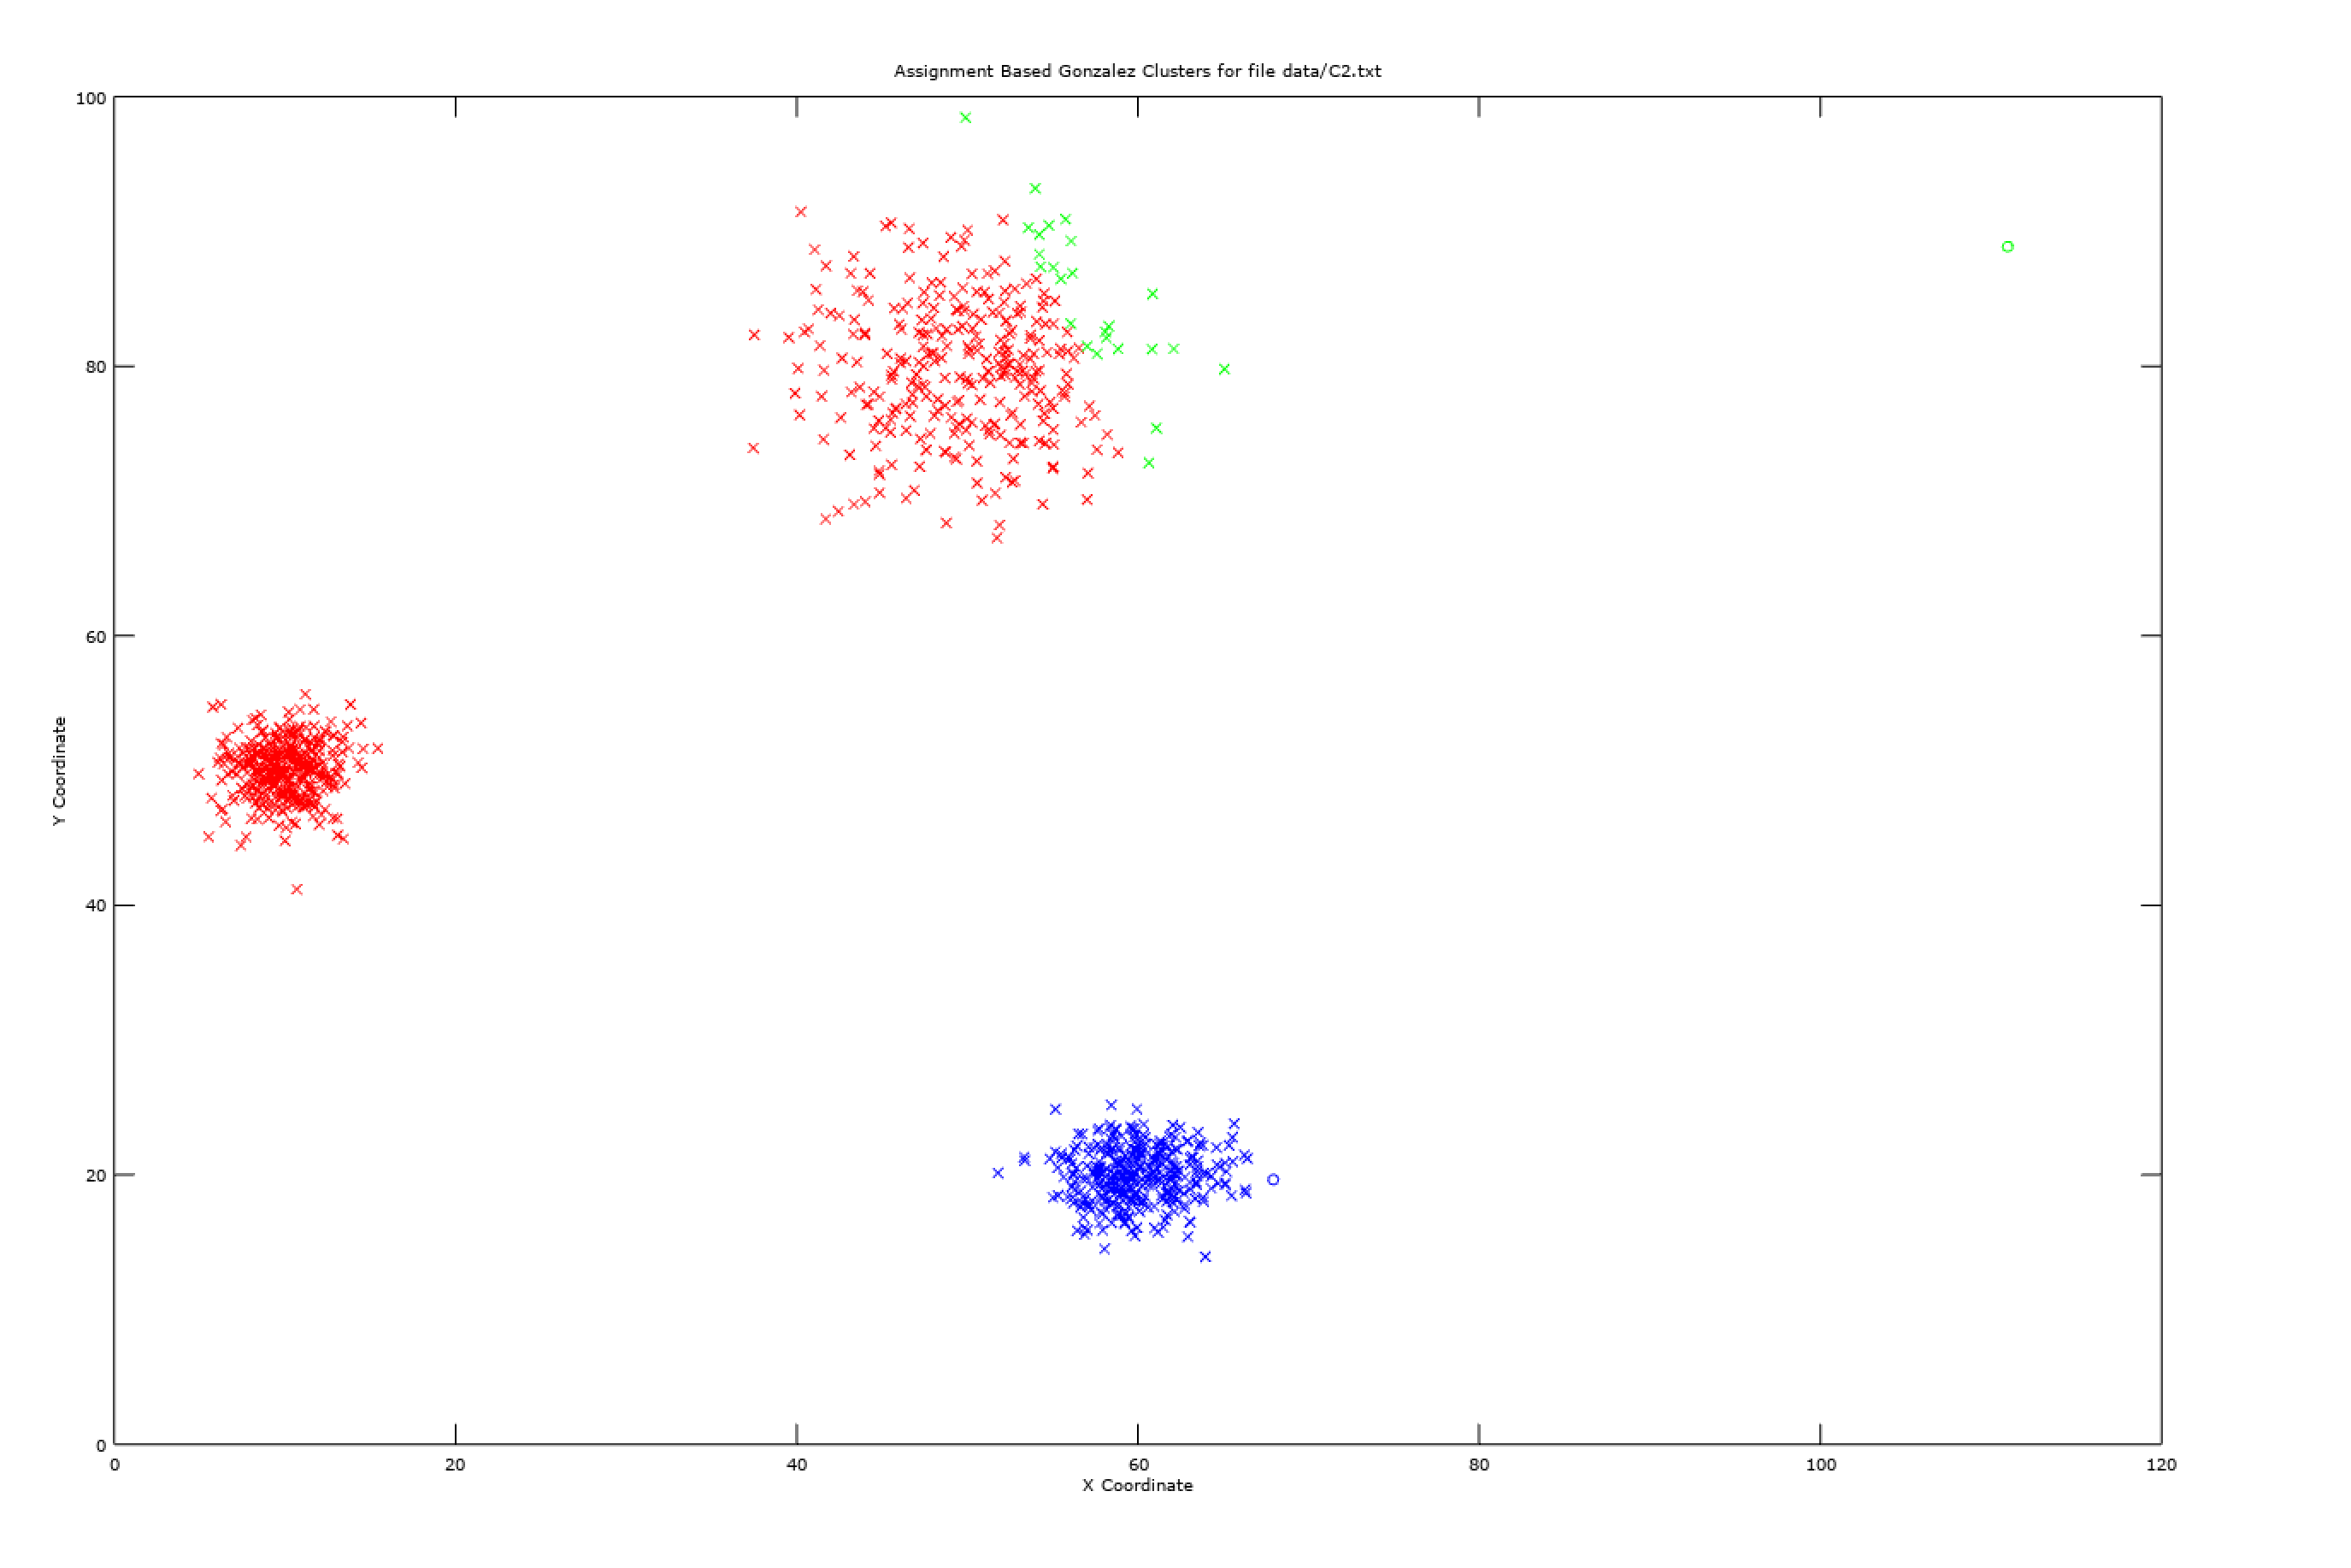
\includegraphics[width=5in]{figures/2AGonzalez.png}
\caption{Gonzalez Clustering}
\label{Gonzalez}
\end{figure}

\begin{figure}[!htb]
\centering
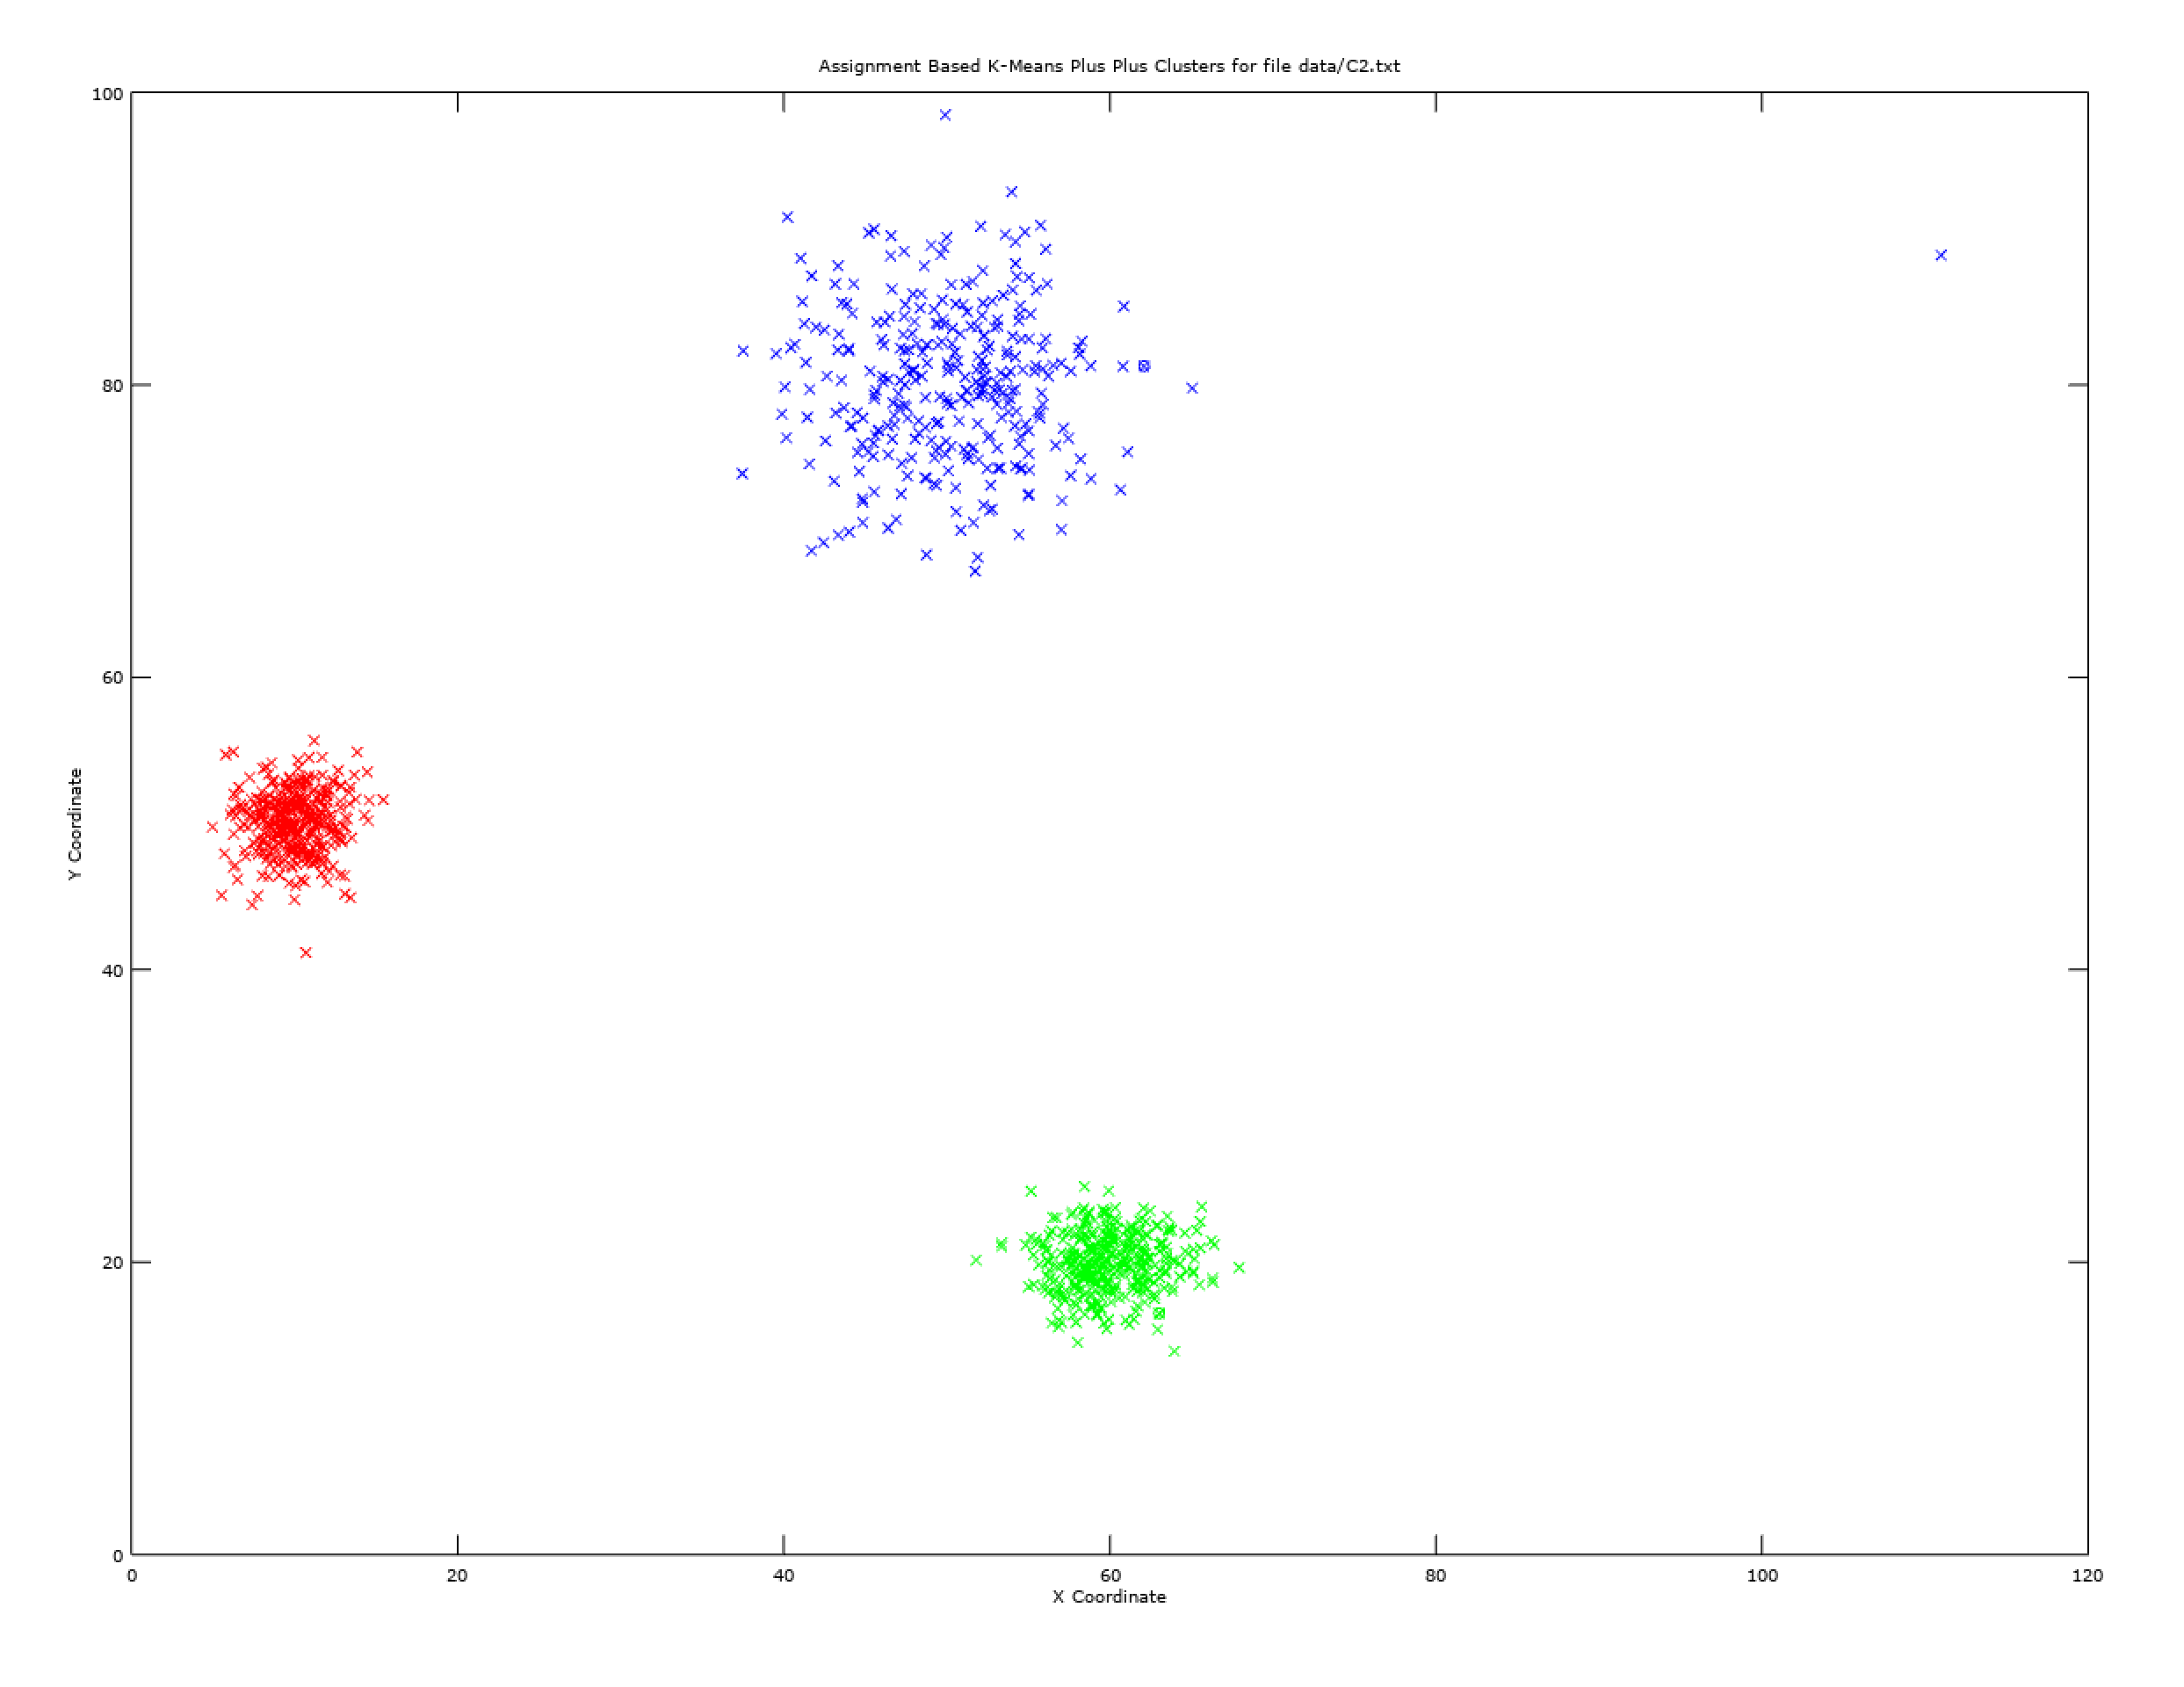
\includegraphics[width=5in]{figures/2AKmeansPP.png}
\caption{K-Means++ Clustering}
\label{KMPP}
\end{figure}

\begin{figure}[!htb]
\centering
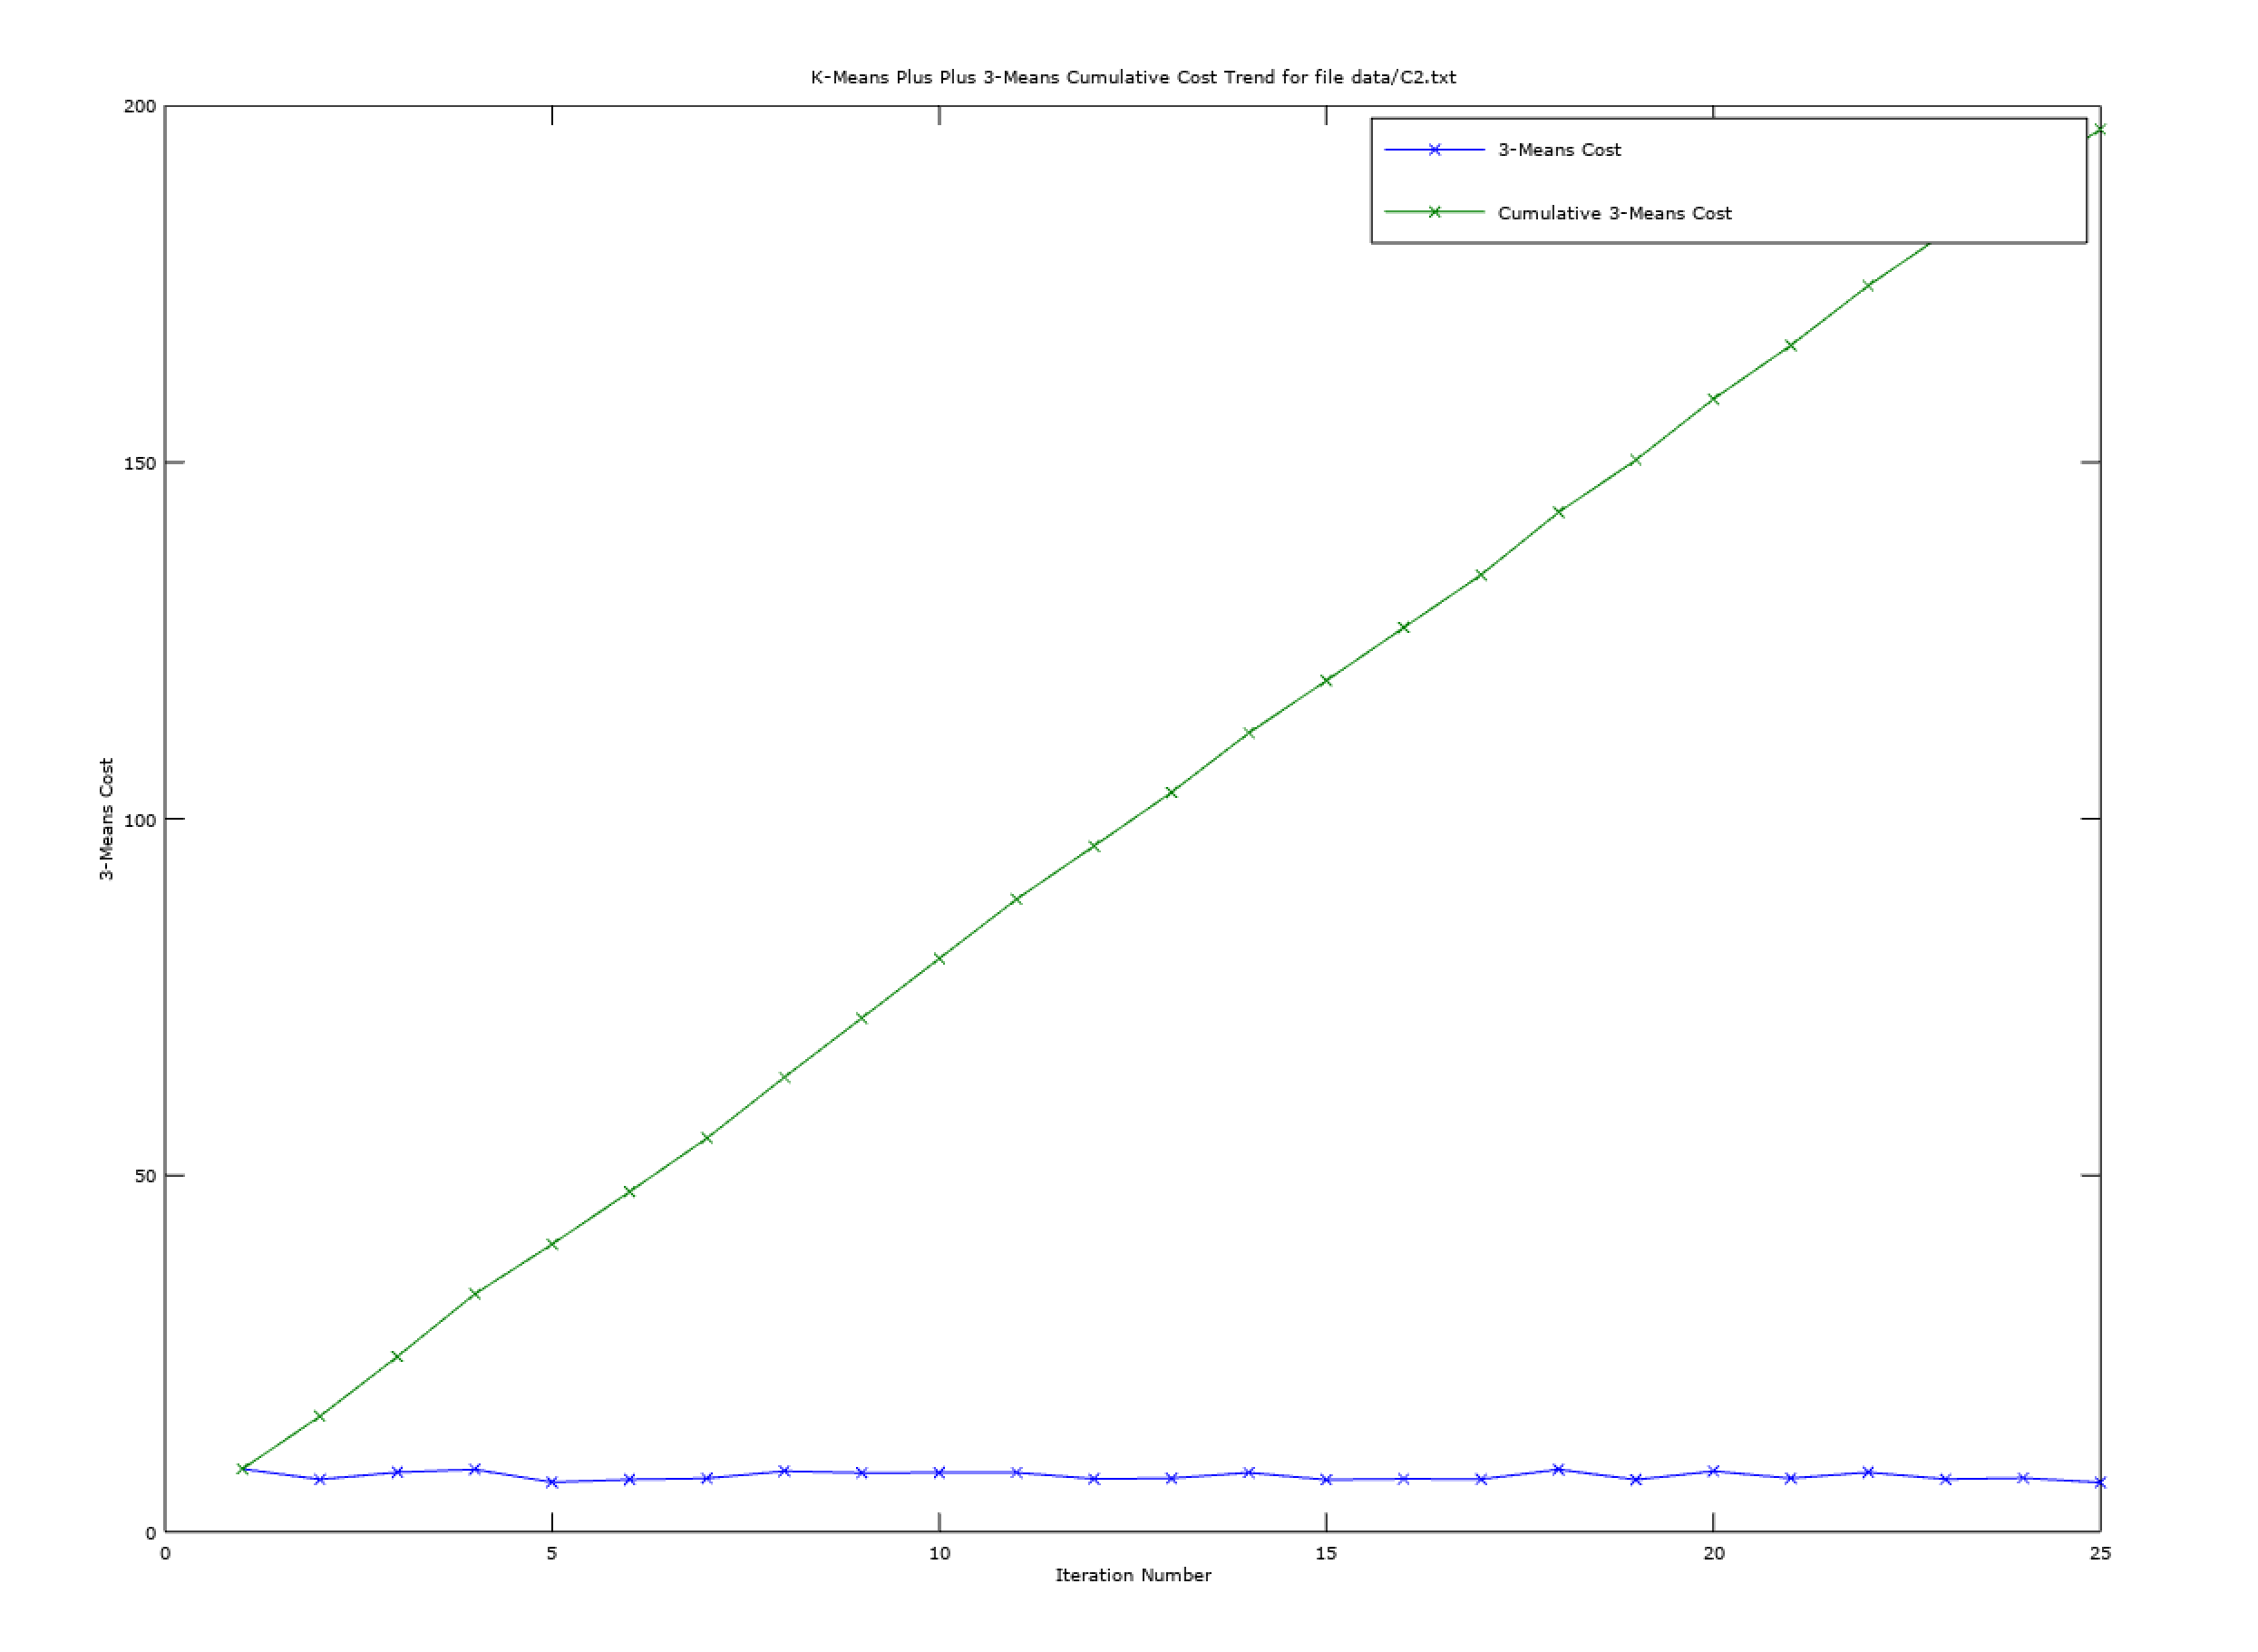
\includegraphics[width=5in]{figures/2AKMPPCum.png}
\caption{K-Means++ 3-Means cost and cumulative cost trend}
\label{KPPCum}
\end{figure}

\begin{figure}[!htb]
\centering
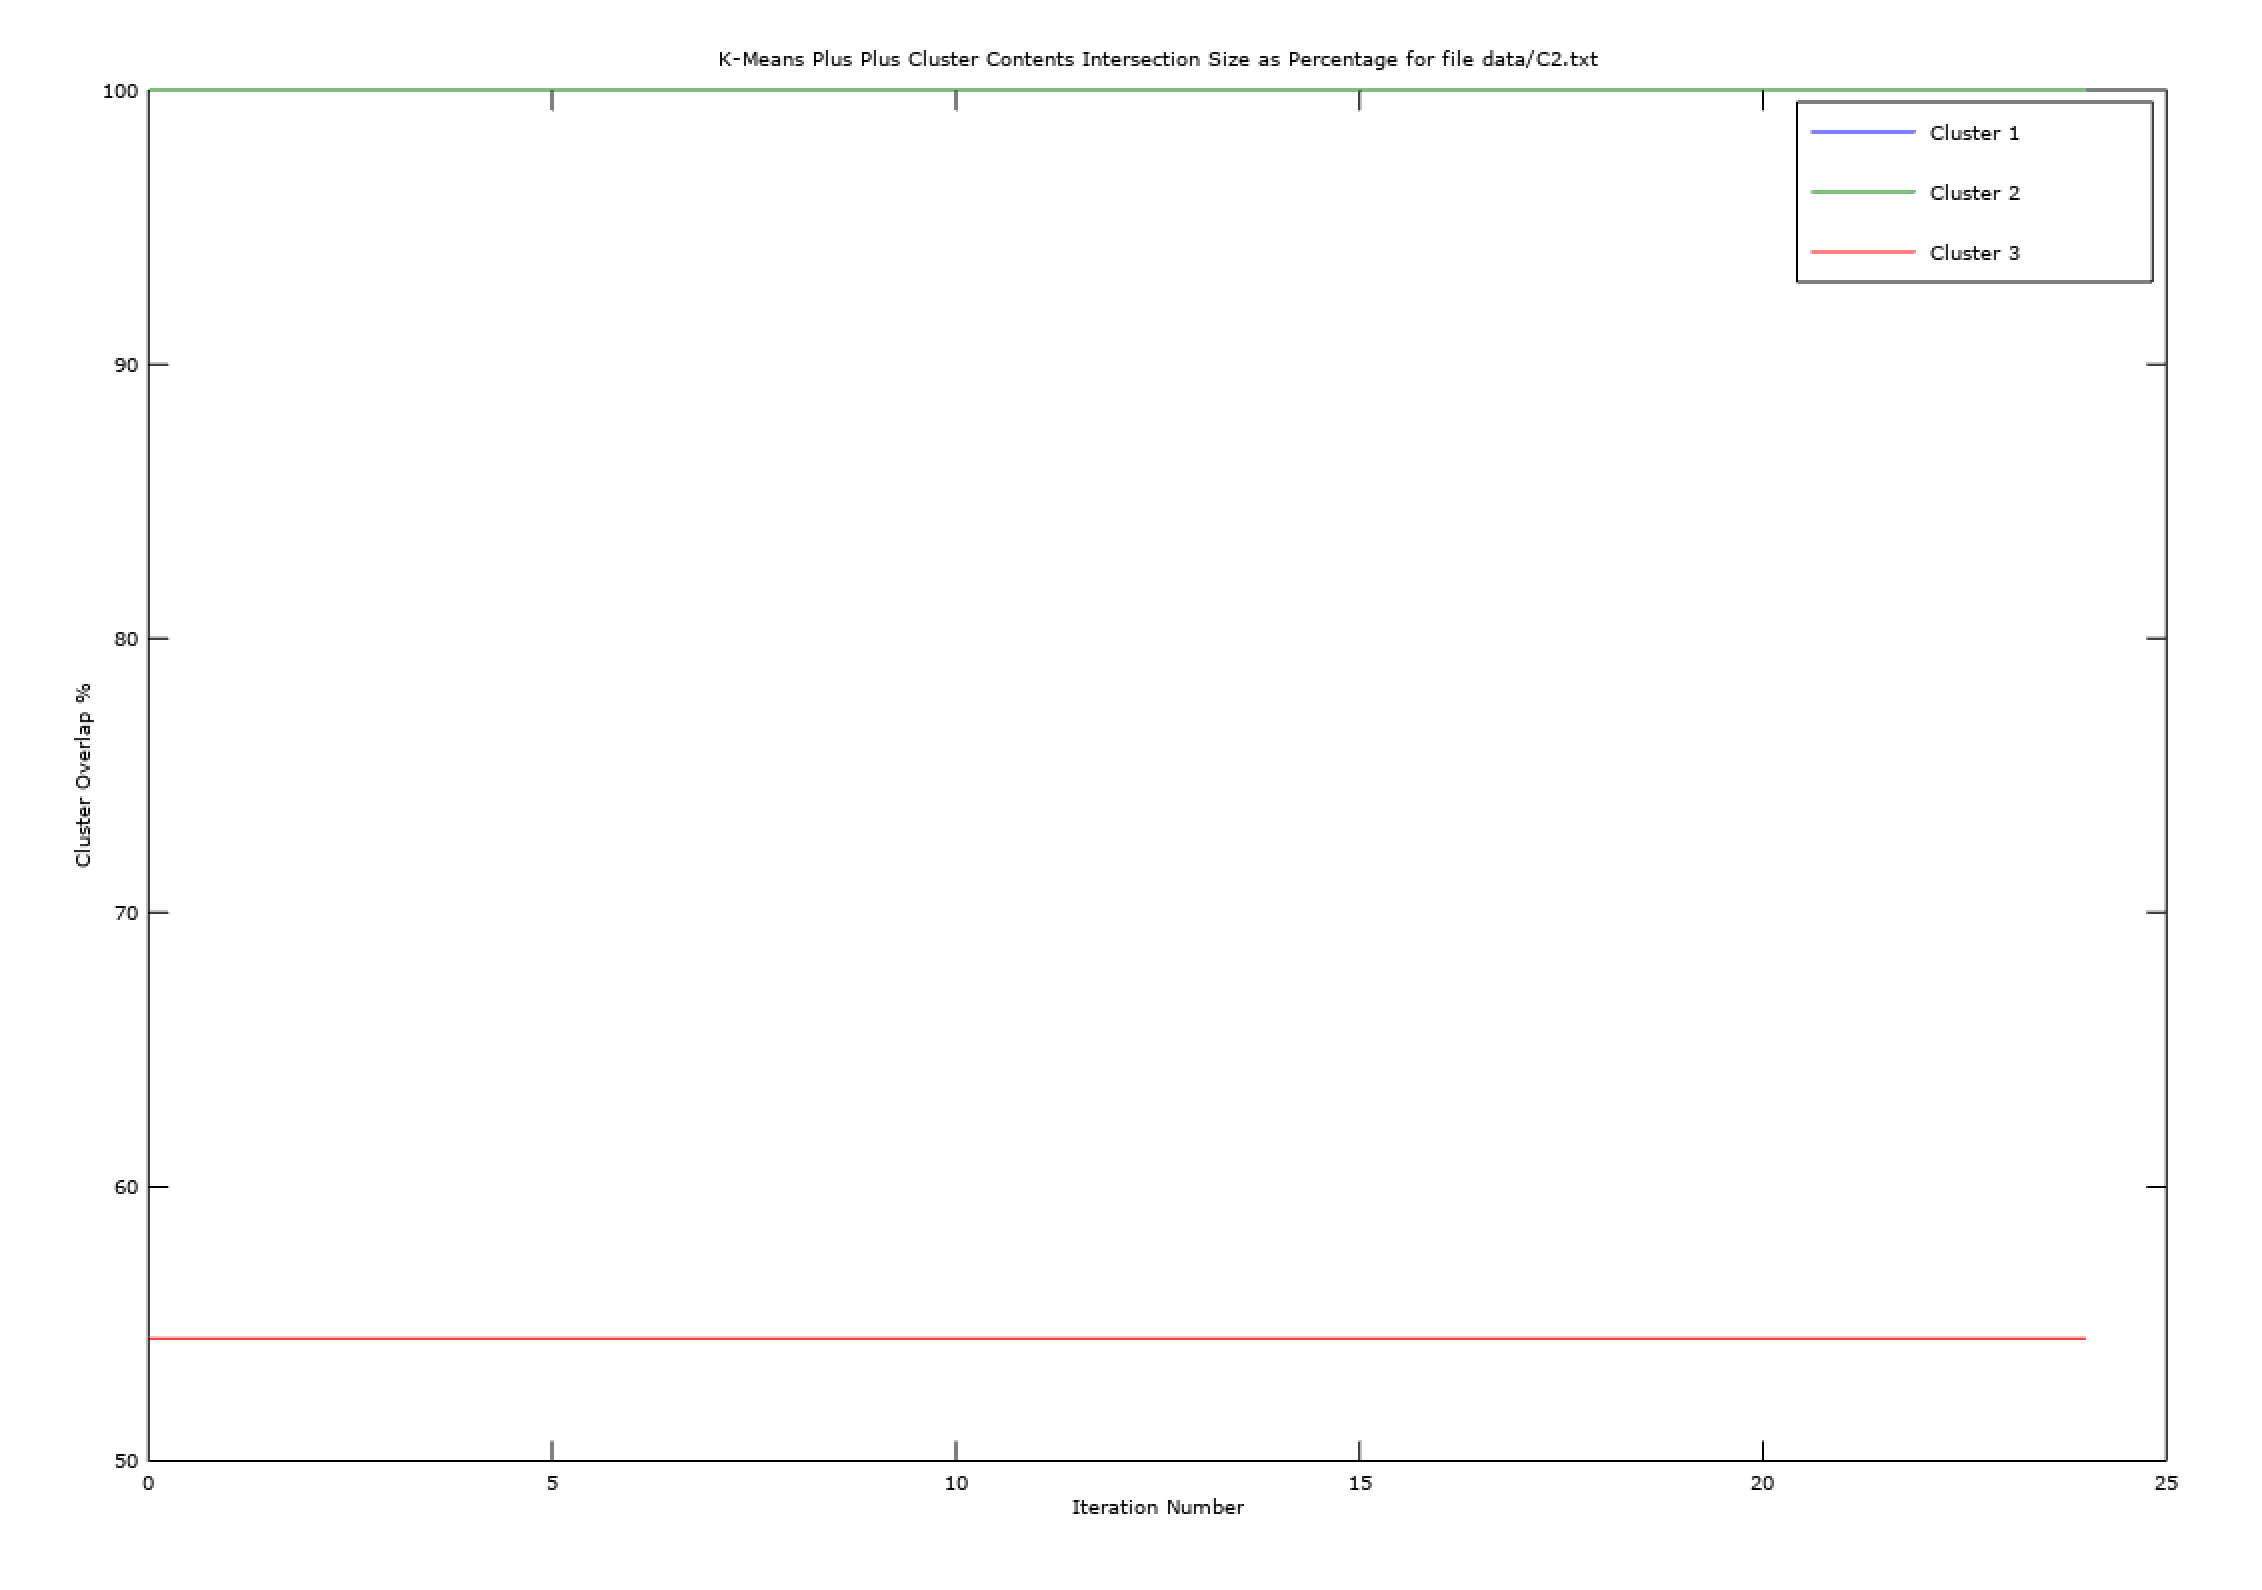
\includegraphics[width=5in]{figures/2AOverlap.png}
\caption{Cluster overlap \% between Gonzalez and K-Means++}
\label{2BOverlap}
\end{figure}

\paragraph{B: (20 points)} 

\begin{figure}[!htb]
\centering
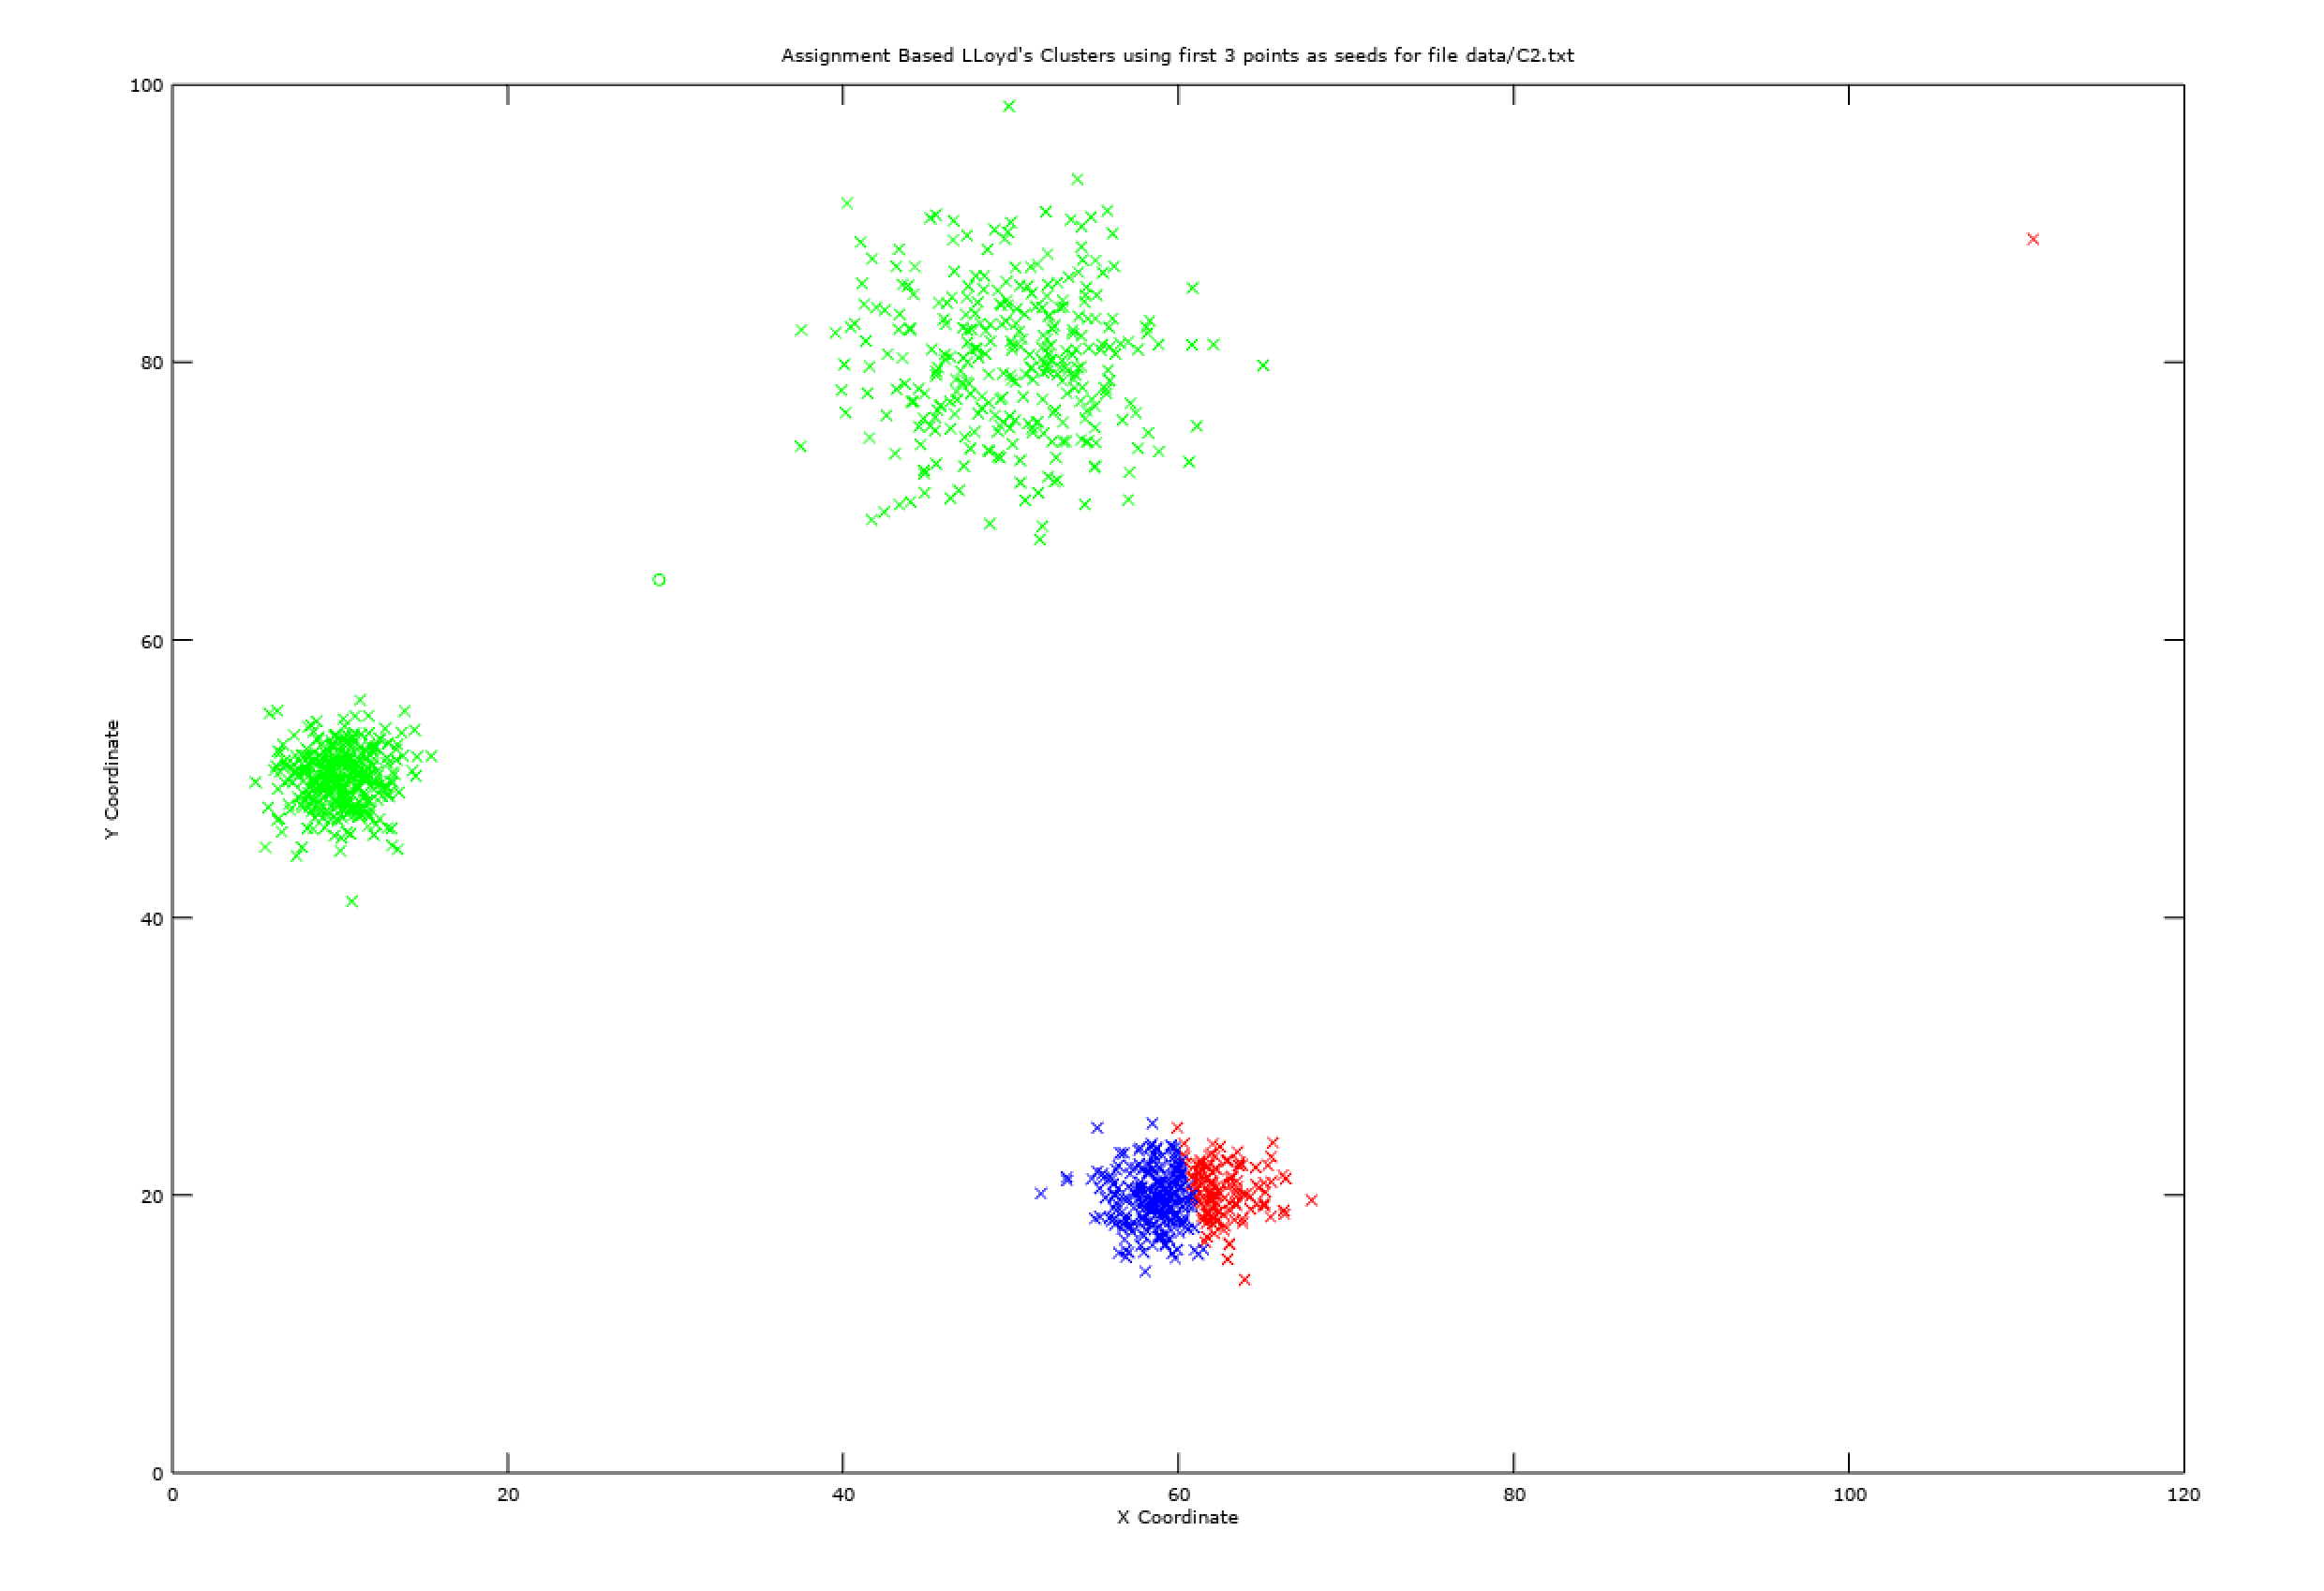
\includegraphics[width=5in]{figures/2BLloydsS3.png}
\caption{Lloyds algorithm with first three points as seeds}
\label{2BLloydS3}
\end{figure}

\begin{figure}[!htb]
\centering
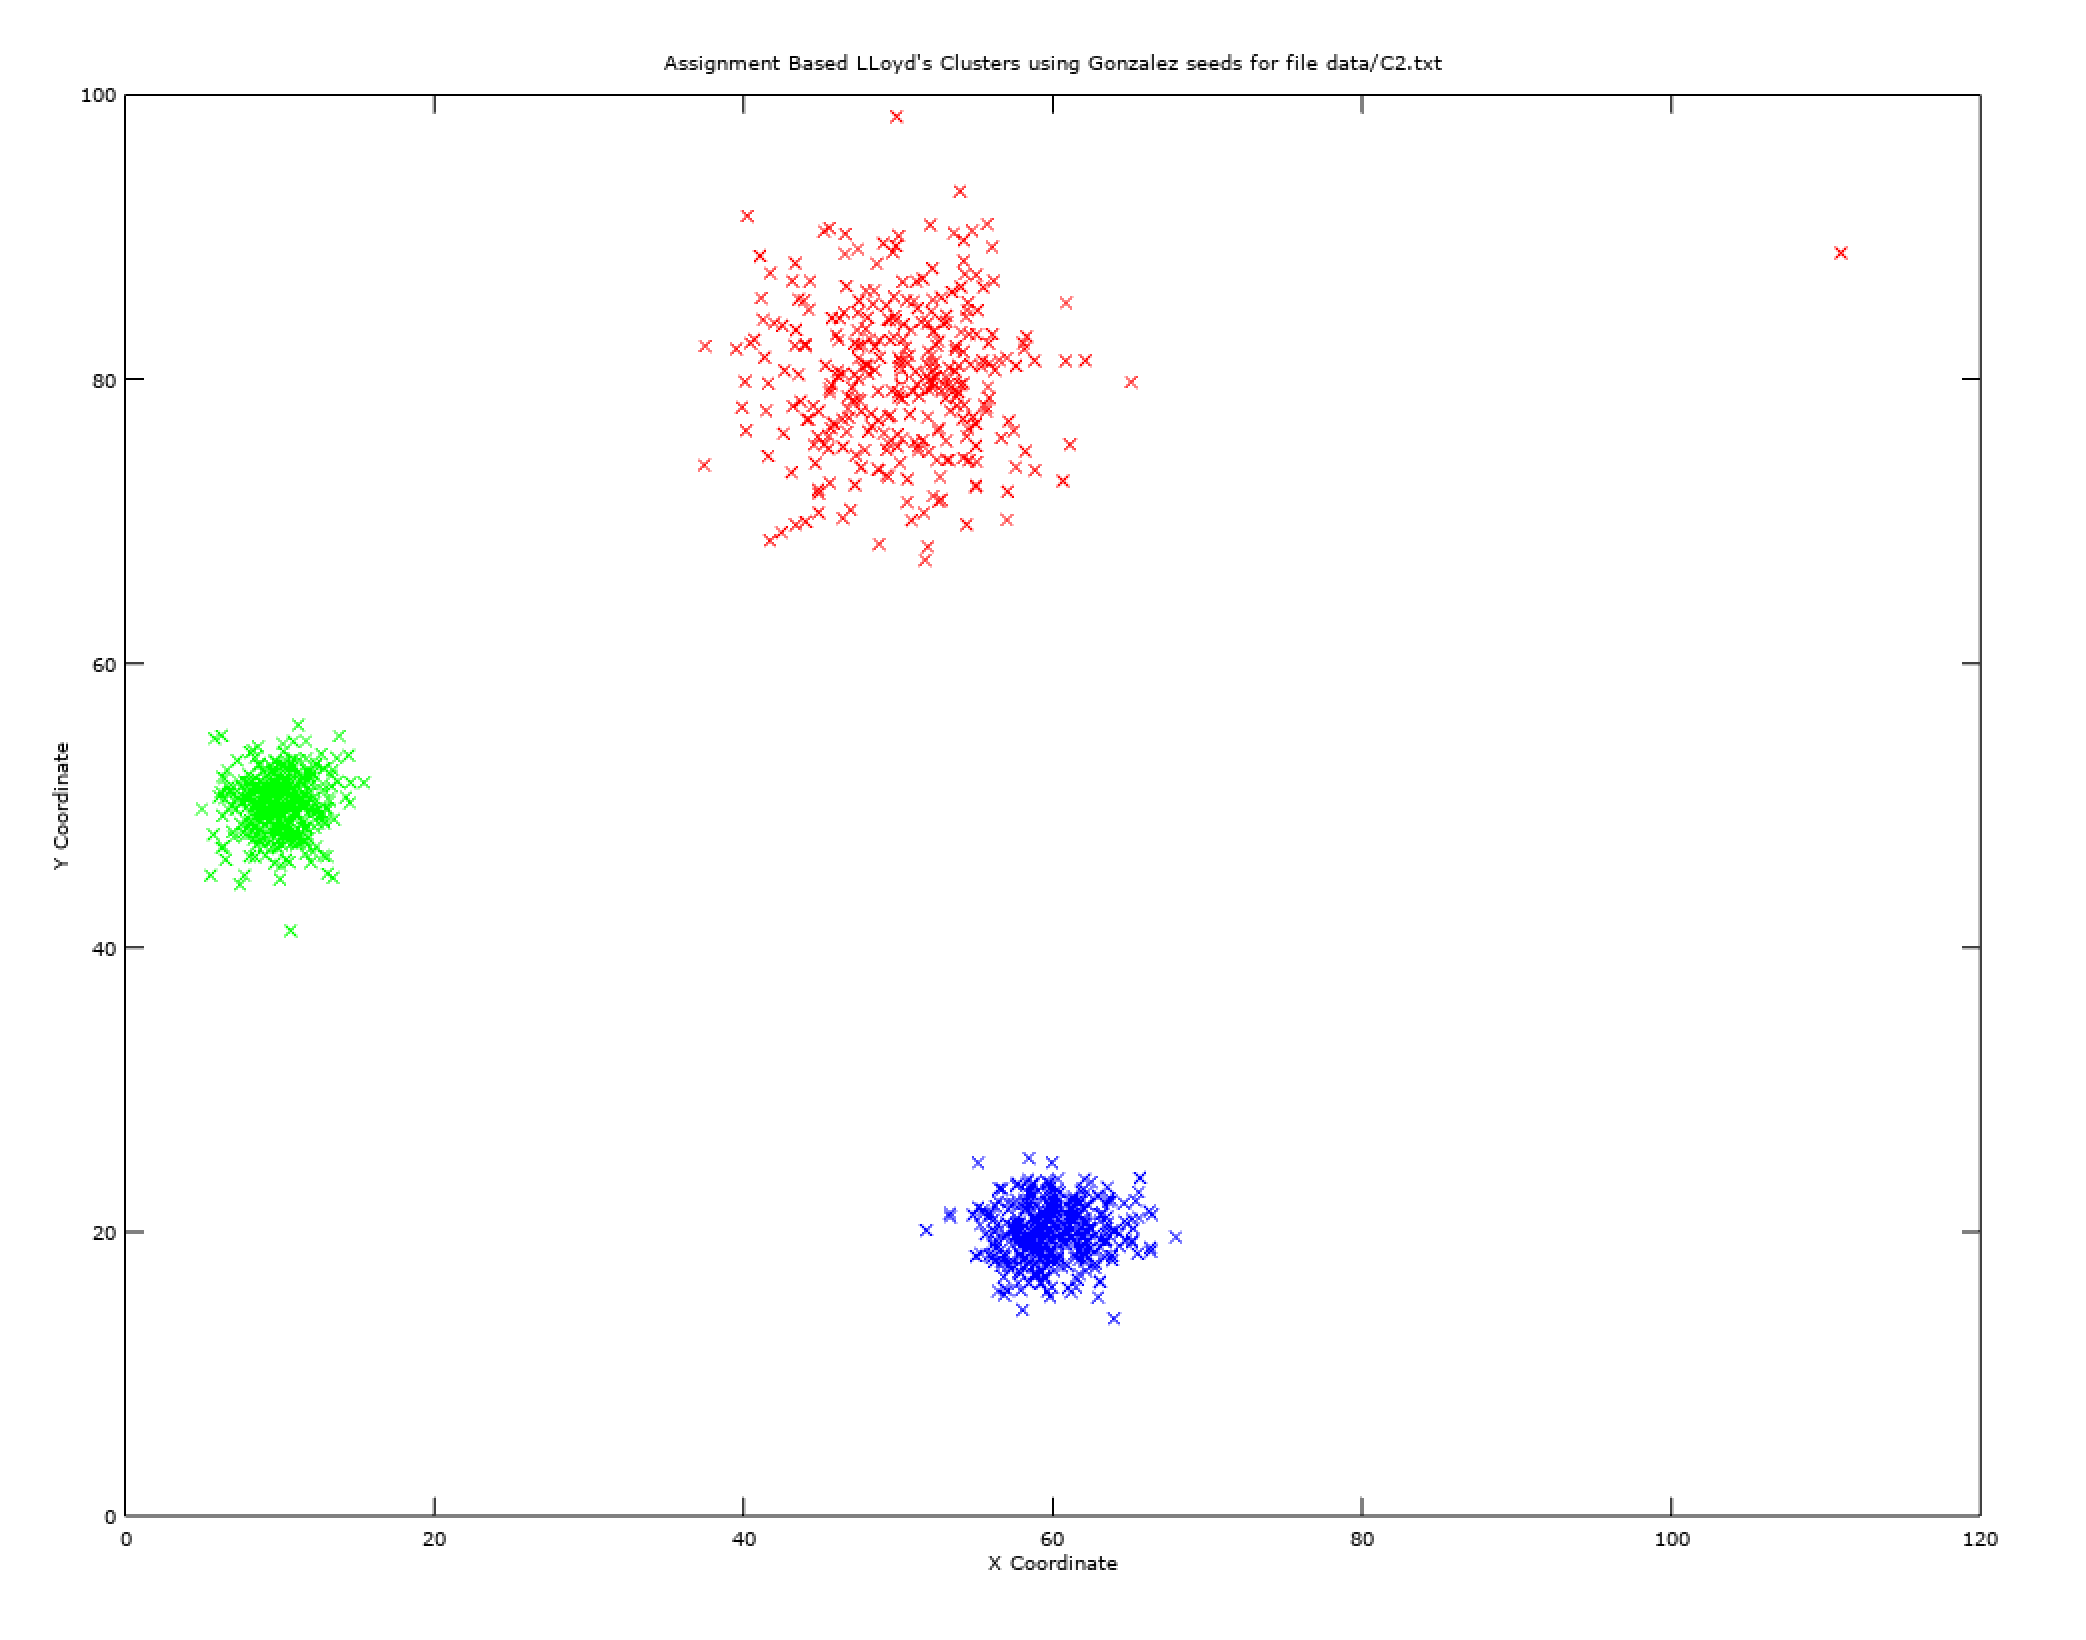
\includegraphics[width=5in]{figures/2BLloydsGSeed.png}
\caption{Lloyds algorithm with Gonzalez Cluster Centers as seeds}
\label{2BLloydsGSeed}
\end{figure}

\begin{figure}[!htb]
\centering
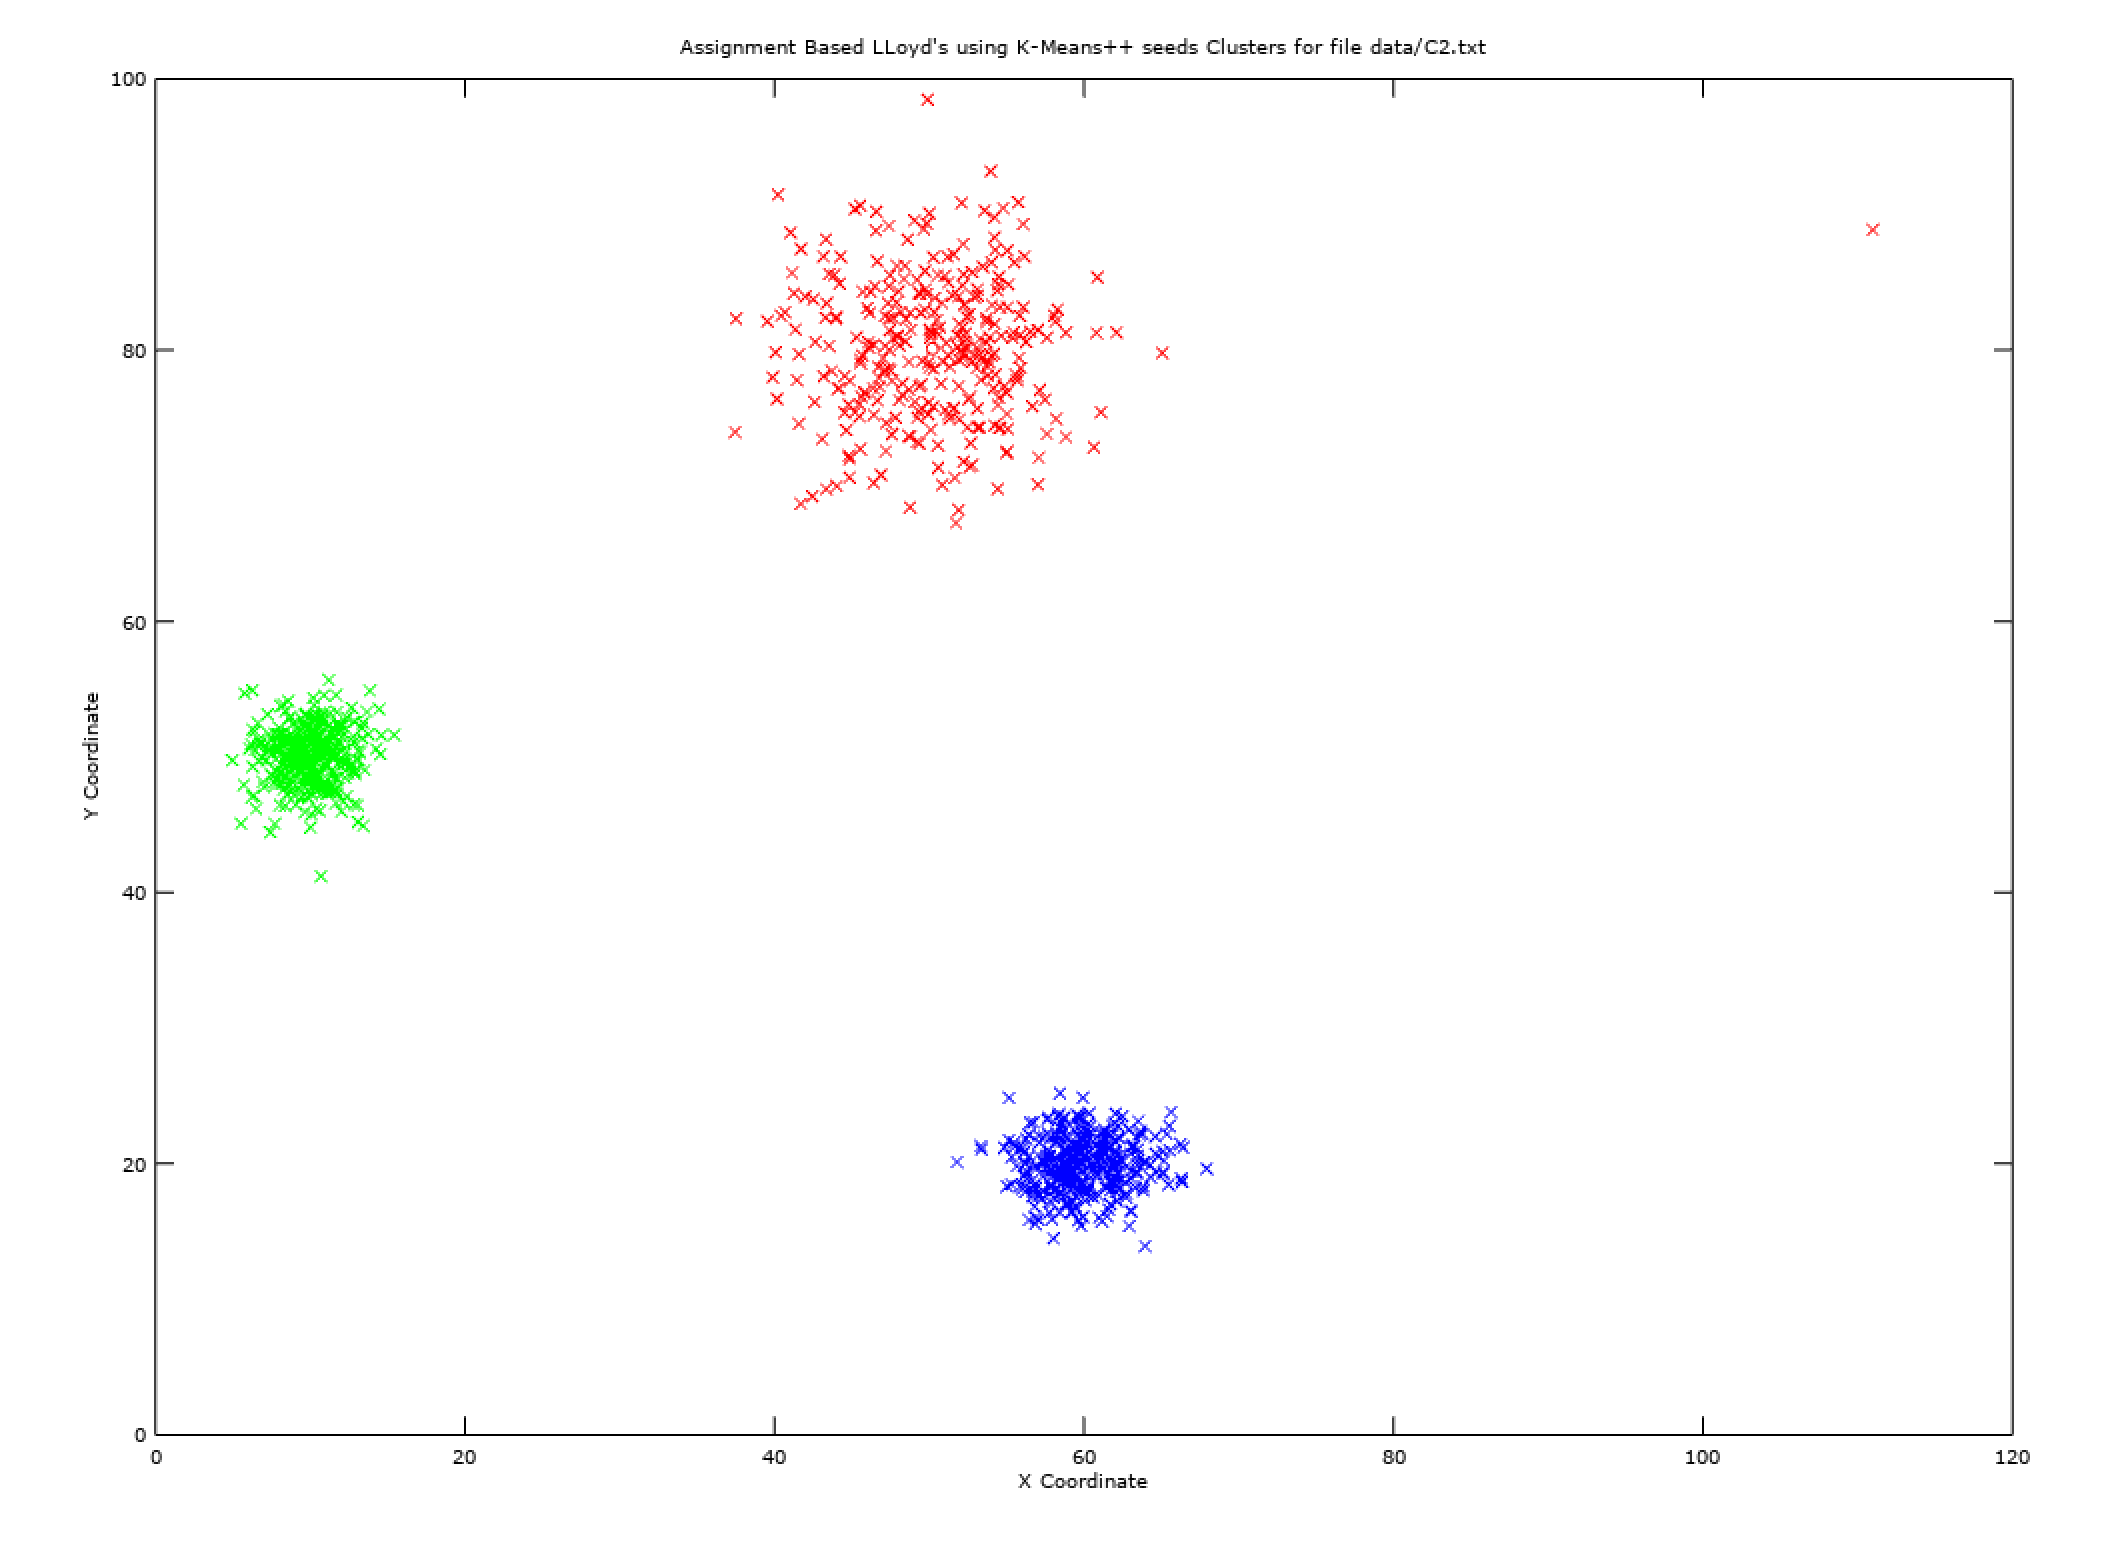
\includegraphics[width=5in]{figures/2BLloydsKMPPSeed.png}
\caption{Lloyds algorithm with K-Means++ Centers as seeds}
\label{2BLloydsKMPPSeed}
\end{figure}

The clusters for Lloyds algorithm using the first $3$ points in file C2.txt as seeds, is shown in figure \ref{2BLloydS3}. \\

The clusters for Lloyds algorithm using Gonzalez Cluster Centers as seeds, is shown in figure \ref{2BLloydsGSeed}. This has much better results as the seeds provided were better.\\

The clusters for Lloyds algorithm using K-Means++ Cluster Centers as seeds, is shown in figure \ref{2BLloydsKMPPSeed}. This also has much better results when compared to the case with the first three points in the file as seeds.\\

In the last two cases, the resulting clusters had exactly the same centers and consequently identical 3-Means costs.\\ 

The centers and 3-Means costs associated with each run of Lloyds algorithm with a different seed is shown in table \ref{table:coords2}.\\

In the case of the run of Lloyds algorithm, where the seed was the centers produced by K-Means++, as shown in figure \ref{2BOverlap}, the cluster contents are exactly the same for each iteration as in the case of the K-Means++ run. This is probably because the clusters converged in the first iteration due to the good seed. Since the three lines overlap, only one line is visible in the figure.

    \begin{table}[!h] 
    \centering
    \caption{Lloyds Algorithm - Coordinates for cluster centers}
    \label{table:coords2}
    \begin{tabular}{|c|c|c|c|c|}
      \hline
   Seeds  & Red  Cluster&  Green Cluster & Blue Cluster & 3-Means Cost \\
      \hline      
      $1^{st}$ 3 points &   $(63.0104, 20.8551)$              &  $(29.0268, 64.3341)$  &          $(58.4236, 19.7766)$            & $20.7920$                     \\
\hline      
      Gonzalez Centers&   $(50.2172, 80.1006)$              &  $(9.9968, 50.0686)$  &          $(59.9465, 19.9731)$      & $5.0322$                     \\
      \hline      
      K-Means++ Centers&    $(50.2172, 80.1006)$             & $(9.9968, 50.0686)$   &           $(59.9465, 19.9731)$  &  $5.0322$                       \\
      \hline      
    \end{tabular}
    \end{table}
 
\begin{figure}[!htb]
\centering
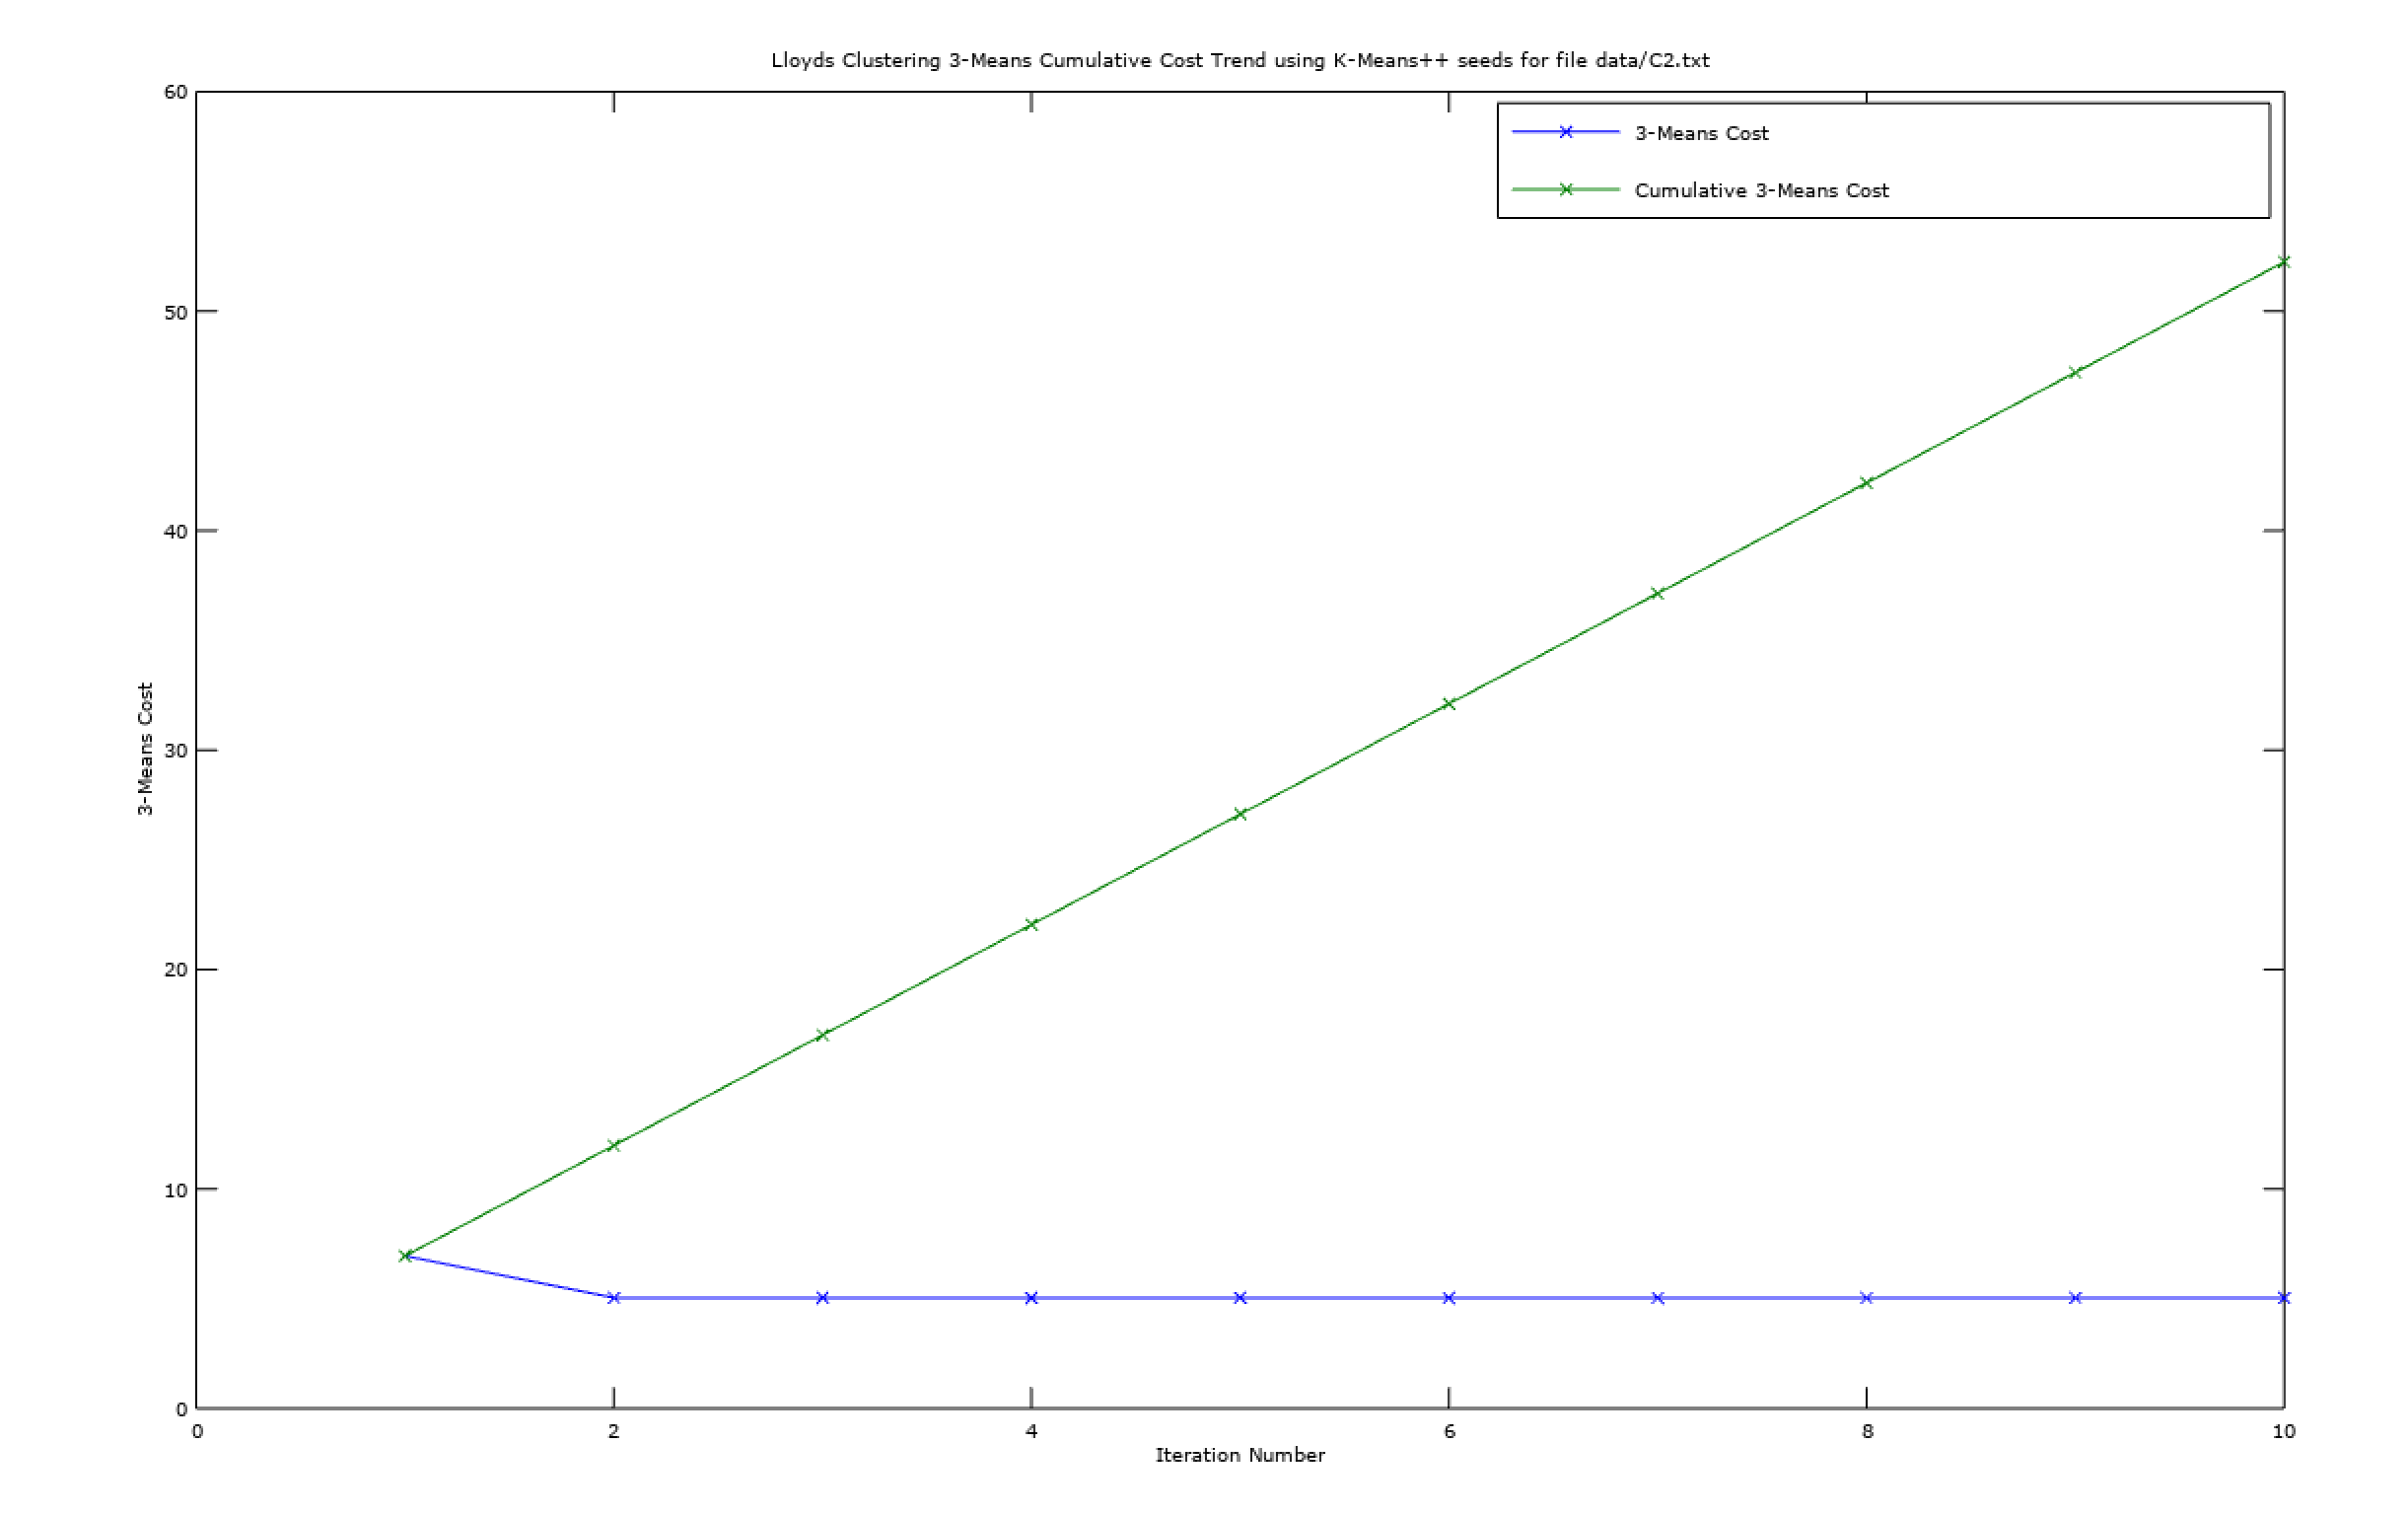
\includegraphics[width=5in]{figures/2BLloydsCum.png}
\caption{Lloyds algorithm with K-Means++ Centers as seeds 3-Means cost and cumulative cost trend}
\label{2BLloydsCum}
\end{figure}

\begin{figure}[!htb]
\centering
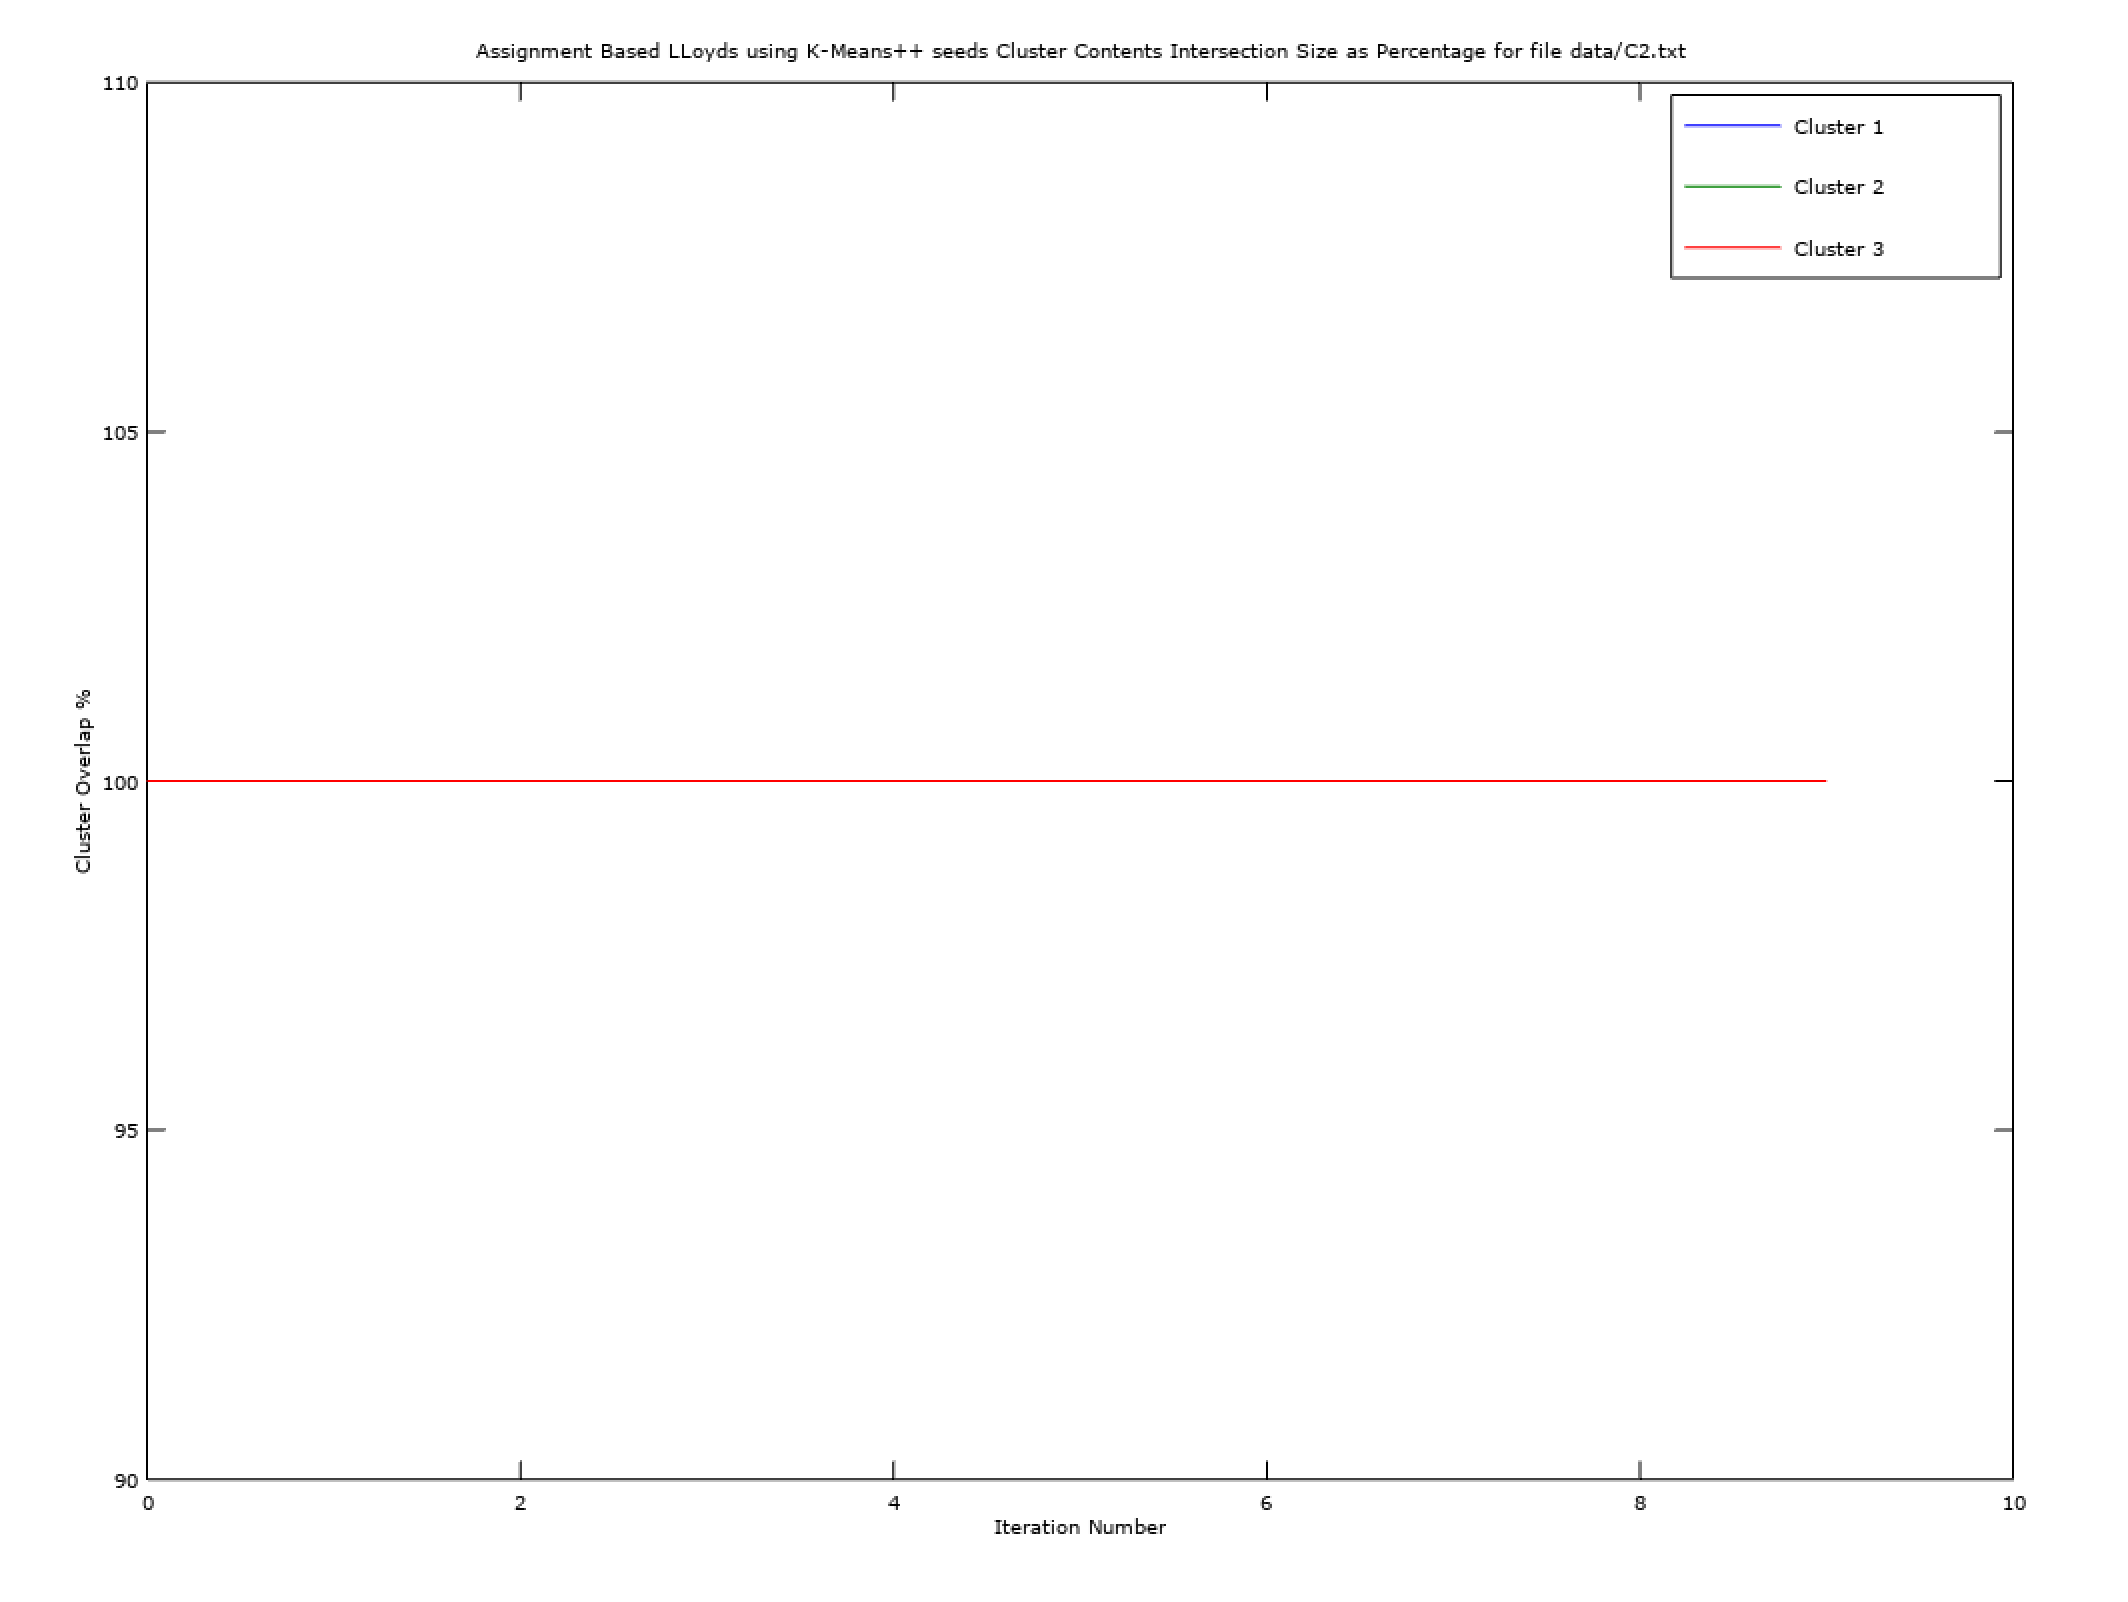
\includegraphics[width=5in]{figures/2BOverlap.png}
\caption{Cluster overlap \% between K-Means++ and Lloyds}
\label{2BOverlap}
\end{figure}

\section{High-dimensional Distances (15 points)}

Let $r'=cr$ be the radius the sphere needs to have, in order for its volume to match the volume of the smallest box that contains it in $d$ dimensions. Here $r$ is the radius of the sphere and $2r$ is the length of one side of the smallest box that contains the sphere. This means that:\\

\begin{equation*}
\begin{aligned}
(2r)^d &= \frac{\pi^{\frac{d}{2}}}{\Gamma \left (\frac{d}{2} +1 \right )} (cr)^d  \\
2^d &= \frac{\pi^{\frac{d}{2}}}{\Gamma \left (\frac{d}{2} +1 \right )} c^d  \\
c &= \left ( \frac{2^d \Gamma \left ( \frac{d}{2} + 1 \right )}{\pi ^ \frac{d}{2}} \right ) ^ \frac{1}{d}\\
&= 2 \left ( \frac{ \Gamma \left ( \frac{d}{2} + 1 \right )}{\pi ^ \frac{d}{2}} \right ) ^ \frac{1}{d}
\end{aligned}
\end{equation*}

I used the above expression for $c$, the multiple for the center, to write an Octave (open source Matlab equivalent) script to plot the value of $c$ versus $d$. I used the built in $gamma$ function in Octave. The plot is shown in figure \ref{cplot}.

\begin{figure}[!htb]
\centering
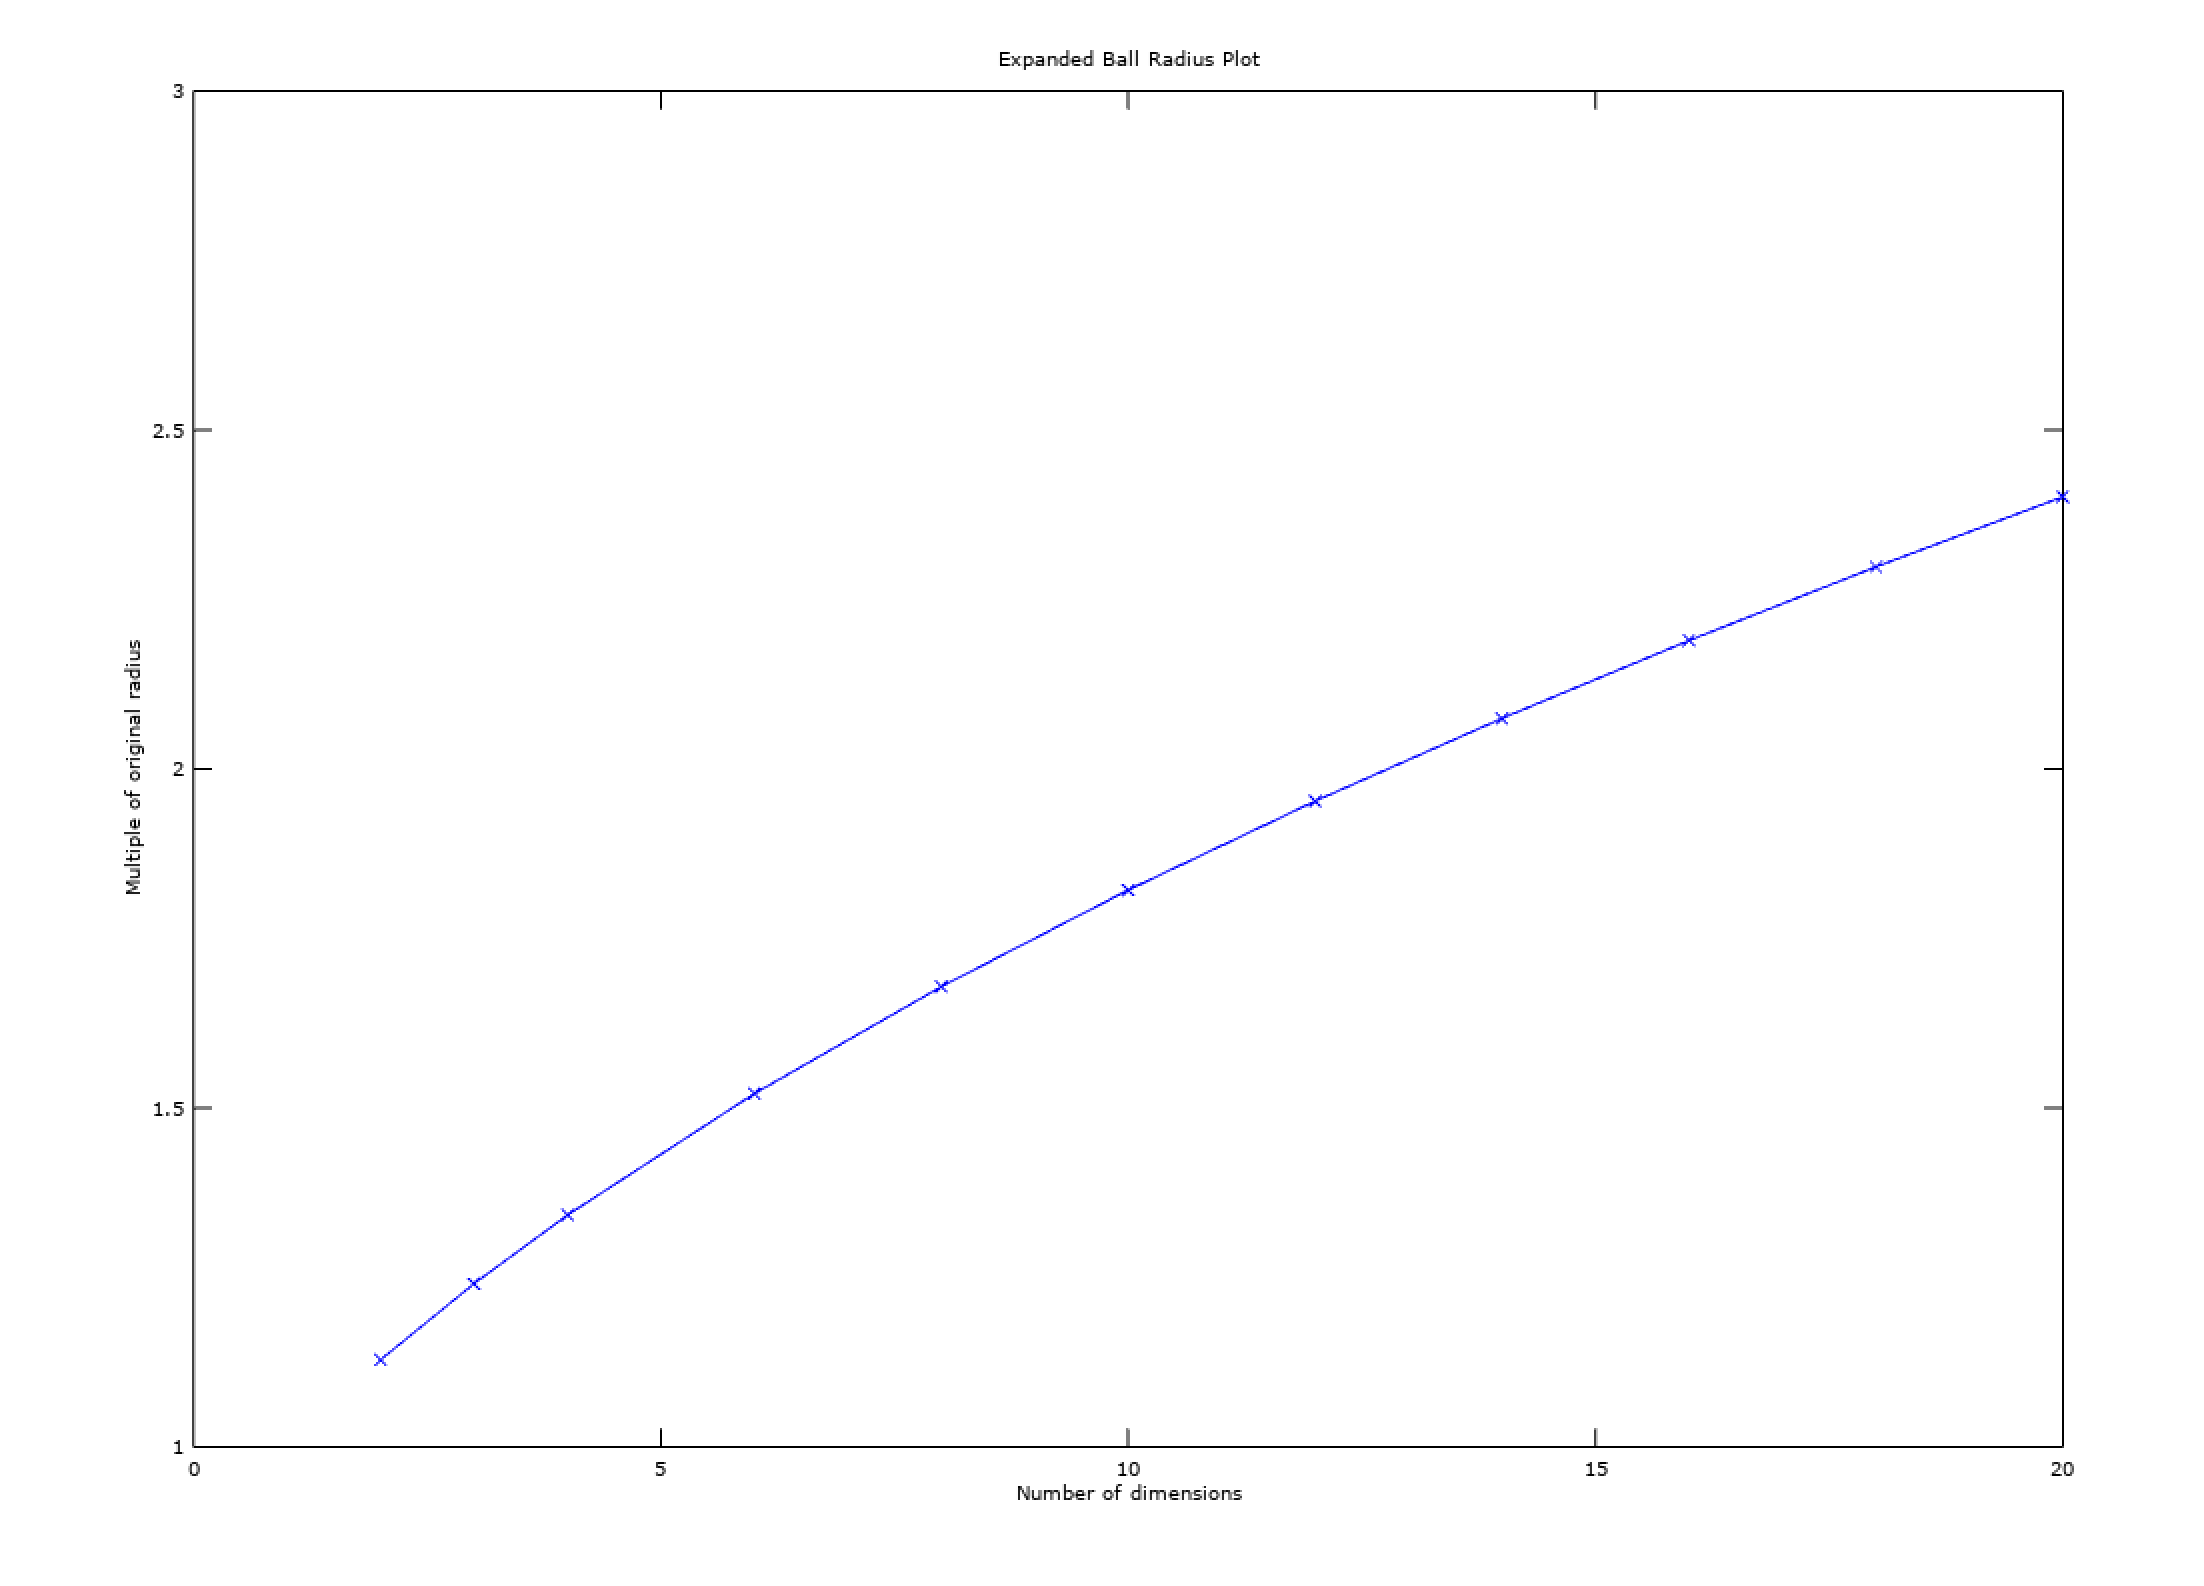
\includegraphics[width=5in]{figures/3cplot.png}
\caption{Sphere radius multiple to match volume of smallest box enclosing it}
\label{cplot}
\end{figure}

\section{$k$-Median Clustering (25 points)}

\paragraph{A: (20 points)} 
Since Lloyds algorithm works by starting with a good seed and running multiple iterations where the new center for each cluster is computed by finding the average of each point in a cluster, I reasoned that this will have the effect of minimizing the median cost. So I decided to use the output of Gonzalez clustering as the seed for running Lloyds algorithm on the data for finding $4$ clusters. I got a Manhattan 4-Median cost of $1.1145$ by finding the sum of the Manhattan distance between each point and its center and then dividing the total by the number of points. The 4-Median Euclidian cost was $0.6025$. The centers produced are being submitted with this report.

\paragraph{B: (5 points)}
I obtained a Manhattan 5-Median cost of $0.8516$ and a Euclidian 5-Median cost of $0.4616$ after running the same setup as above for 5 clusters. The centers found are shown in table \ref{table:centers}

    \begin{table}[!h] 
    \centering
    \caption{Centers for 5 clusters found by running $5$-Median clustering on C3.txt}
    \label{table:centers}
    \begin{tabular}{|c|c|}
      \hline
   Center  & Coordinates \\
      \hline      
      $1$ &   $(1.004409000, 0.002728689, -0.030692661, 0.006958770, 0.009213202)$ \\
    \hline      
      $2$ &   $(-0.008042136, -0.011766920, 0.010481614, 0.995836267, -0.048693795)$\\
    \hline      
      $3$ &   $(0.027419583, -0.000930982, 1.021313969, 0.014982278, -0.006411439)$ \\
    \hline      
      $4$ &   $(0.001010261, 1.006812335, 0.016194060, -0.003527564, -0.011586995)$\\
    \hline      
      $5$ &   $(0.022707830, -0.010666050, -0.004099600, -0.006732945, 1.013415380)$\\
    \hline      
    \end{tabular}
    \end{table}

 
\end{document}
